% TIPS FROM JOHN
% Don't mix levels of abstraction 
% You should be able to understand the report just by reading the section headings, just at a coarser level of detail.
% Each part of your report should logically follow from the previous.
% Use a consistent tense and voice.
% Define abbreviations, symbols and use and capitalise them consistently
% to specifically attribute You must cite anything you quote or take imagery from, or otherwise directly use ideas from, or you are committing plagiarism.
% to discuss ideas from Cite texts that contribute to your arguments. You need to show you are aware of, and can comment critically on work done by others.
% to provide background Cite texts that providing supporting material. For example, don't explain to the reader how a recurrent neural network works in the form of a tutorial. This isn't your job. Instead, briefly describe it and refer to a citation for further details.



% REMEMBER: You must not plagiarise anything in your report. Be extremely careful.

\documentclass{l4proj}

    
%
% put any additional packages here
%

\begin{document}

%==============================================================================
%% METADATA
% Inverse-Problems and Generative Models for Artificial Colouring and Image Restoration
% Machine learning methods to solve the inverse problem of image colourisation
\title{Deep Learning Methods to Solve the Inverse Problem of Artificial Image Colourisation}
\author{James Conway}
\date{April 6, 2020}

\maketitle

%==============================================================================
%% ABSTRACT
% Abstract is formulaic:
% Motivate; set aims; describe; explain results
% "XYZ is bad. This project investigated ABC to determine if it was better. ABC used XXX and YYY to implement ZZZ. It was found that ABC was better than XYZ, though it caused rabies in half of subjects."
% Colourisation is a difficult and ambiguous problem, the solution of which needs to account for a large amount of information, which is something Deep Learning excels at. This project aims to investigate which Deep Learning models in particular are best suited for colourisation

\begin{abstract}
    To-Do
\end{abstract}

%==============================================================================

% EDUCATION REUSE CONSENT FORM
% If you consent to your project being shown to future students for educational purposes
% then insert your name and the date below to  sign the education use form that appears in the front of the document. 
% You must explicitly give consent if you wish to do so.
% If you sign, your project may be included in the Hall of Fame if it scores particularly highly.
%
% Please note that you are under no obligation to sign 
% this declaration, but doing so would help future students.
%
\def\consentname {James Conway} % your full name
\def\consentdate {6 April 2020} % the date you agree
%
\educationalconsent


%==============================================================================
\tableofcontents

%==============================================================================
%% Notes on formatting
%==============================================================================
% The first page, abstract and table of contents are numbered using Roman numerals and are not
% included in the page count. 
%
% From now on pages are numbered
% using Arabic numerals. Therefore, immediately after the first call to \chapter we need the call
% \pagenumbering{arabic} and this should be called once only in the document. 
%
% Do not alter the bibliography style.
%
% The first Chapter should then be on page 1. You are allowed 40 pages for a 40 credit project and 30 pages for a 
% 20 credit report. This includes everything numbered in Arabic numerals (excluding front matter) up
% to but excluding the appendices and bibliography.
%
% You must not alter text size (it is currently 10pt) or alter margins or spacing.
%
%
%==================================================================================================================================
%
% IMPORTANT
% The chapter headings here are **suggestions**. You don't have to follow this model if
% it doesn't fit your project. Every project should have an introduction and conclusion,
% however. 
%
%==================================================================================================================================
\chapter{Introduction}

% reset page numbering. Don't remove this!
\pagenumbering{arabic} 

% Should introduce the problem and state your contributions.
% Don’t describe the complexity of the problem in a general sense which your paper clearly won’t solve, concentrate on a more interesting part of it which it does, making it believable that you might solve it.
% Your introduction should make claims then the body of the paper should provide substantiation or evidence to support each claim.

% Introduction: Motivate first, then state the general problem clearly

\section{Motivation}

The most reliable current methods for colourising black and white images involve a mostly manual process, whereby an artist analyses the semantic details of a greyscale image, and from them infers the corresponding colours. This process is often assisted by semi-automatic colourisation tools which are still heavily reliant on user input. Even with such tools, colourisation is still a time-consuming and labour-intensive process, the outcome of which is heavily dependent on the skill of the artist.

The existence of a fully automated tool for colourisation, would allow it to be reliably performed without requiring skilled artists or extensive periods of time. This would mean that projects requiring the colourisation of many numerous images, such as video colourisation, can be carried out far more efficiently than before, and in a fraction of the time. Automatic colourisation could also have other technical uses which aren't possible with current manual methods. For example, some technologies such as night vision or sonar imaging, which are only capable of producing monochromatic images, could use automatic colourisation to make the details of the presented images more noticeable, helping the user to distinguish objects.

\section{Problem and Solution}

Colourisation is part of a particular category of problems known as "ill-posed inverse problems". This means it doesn't have a single direct solution which depends continuously on the provided data, and that it's impossible to formulate a single unique model which is capable of correctly colouring any image. The best way to solve it is by exploiting as much additional information as possible, in order to produce a solution that best approximates the correct result. 

Deep Learning has recently been employed as the solution of choice to this problem, as it provides tools that are capable of accounting for much of this additional information, including many unknown variables which a human may not account for. There are a variety of different Deep Learning methods that are well adapted to tasks involving image analysis, and can also be used for colourisation, however it's still uncertain which method can provide the best solution. In this project we will implement and test a number of these different models, and will compare their performance in order to find the best one.

\section{Aim}

The specific aims of this project are to:
\begin{itemize}
    \item Analyse the nature of the problem, in order to understand how Deep Learning in particular can best solve it.
    \item Investigate how to best prepare the training data to be analysed by the Deep Learning models, and see which data works best.
    \item Implement and test a variety of Deep Learning solutions that could be viable, including a:
    \begin{itemize}
      \item Convolutional Neural Network
      \item Generative Adversarial Network
      \item Variational Autoencoder
    \end{itemize}
    \item Evaluate the performance of each solution, and compare them to determine which is the most viable.
\end{itemize}

\chapter{Background}

In this chapter we will analyse the nature of the problem of colourisation and explain the reasoning behind a Machine Learning approach to solving it. We will also highlight seminal projects that have attempted to solve the problem and what they achieved.

\section{Colourisation as an Inverse Problem}
\label{inverse-prob}
We call two problems inverses of one another if the formulation of each involves all or part of the solution of the other. To solve an inverse problem, we need to look at the direct problem from which it derives which will have a cause-effect sequence to compute the unknown effects of known causes. The inverse problem is then solved by reversing this cause-effect sequence to compute the unknown causes of known effects\cite{Inverses}.

In the case of colourisation we can say that greyscale to colour image conversion is the inverse of colour to greyscale conversion, the solution of which can be found by reversing the colour to greyscale transformation. We'll demonstrate this by first solving the problem of colour to greyscale image conversion. Typically, colour images are represented in data using the Red-Green-Blue (RGB) colour model (see figure \ref{fig:rgb}). 
\begin{figure}[H]
    \centering
    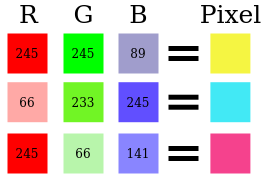
\includegraphics[width=0.5\linewidth]{images/RGB.png}    

    \caption{In the RGB encoding, each pixel's colour value is produced by superimposing Red, Green, and Blue colours of varying intensities.}

    \label{fig:rgb} 
\end{figure}

There is no unique method to perform a RGB to greyscale conversion, however, a common solution is the "Weighted" or "Luminosity" method. This involves multiplying the Red, Green, and Blue values of each pixel by coefficients which represent how much each colour contributes to the overall luminosity of the image, and then summing them together to produce corresponding greyscale pixel values. For instance, if we decided that Red contributes 30\% to the luminosity of an image, Green contributes 59\%, and Blue contributes 11\%, the per-pixel conversion would be as follows:
\begin{equation}
    greyscale = ((0.3 * R) + (0.59 * G) + (0.11 * B))
\end{equation}
However, these channel weightings aren't constant, meaning a loss of information is intrinsic to the conversion from RGB to greyscale. With this loss of information, the inverse problem of then converting from greyscale back to RGB has no unique solution which it can follow to recover the original RGB values. This lack of a unique solution is where the main difficulty of the problem lies, and it puts image colourisation into a particular category known as "ill-posed" inverse problems.

% Finish citations

\section{Ill-posedness}
An ill-posed problem is a problem which violates at least one of Hadamard's three properties of well-posedness\cite{Hadamard}:
\begin{enumerate}
    \item The problem has a solution.
    \item The solution is unique.
    \item The solution depends continuously on the parameters or input data.
\end{enumerate}
Colourisation is ill-posed as it lacks a unique solution and doesn't depend continuously on the input data. A high intensity greyscale pixel can correspond to a high intensity red, green, or blue value, with no discrete information to determine which. No exact algorithm can be developed which is capable of producing correct solutions for any arbitrary input, the only option is to develop an approximate solution.
\begin{figure}[H]
    \centering
    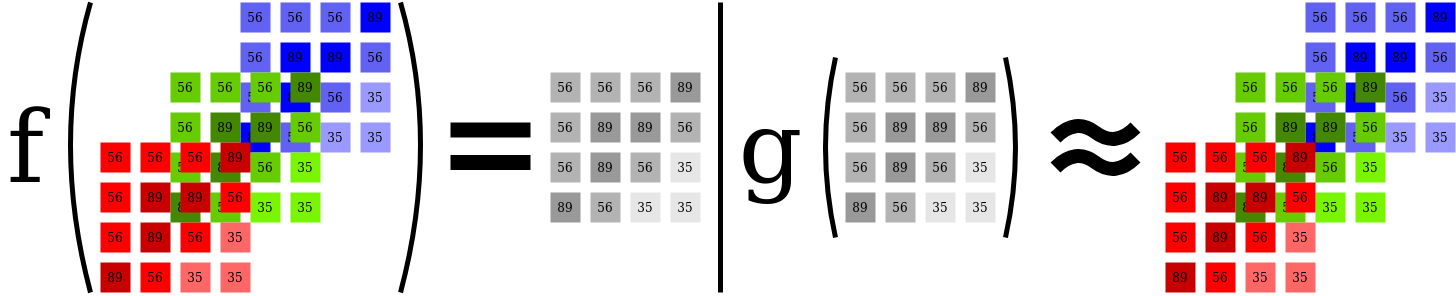
\includegraphics[width=1.0\linewidth]{images/FunctionsHorizontal.png}    

    \caption{With the information lost in the greyscale to colour computation of f, the only solution is to develop a separate function g, capable of producing an approximate computation of f's input.}

    \label{fig:functions} 
\end{figure}

The general rule for finding the best approximate solution is to construct it around additional constraints derived from the nature of the problem, also known as "priors" or "prior information"\cite{Inverses}. There are a multitude of potential priors which can be considered when dealing with colourisation. 

In the context of colourisation, the priors can come in a variety of forms. Low level priors can be very specific details about the image, such as edges and contours, which can indicate where an object and its colours end. High level priors are more general details, like object categories, which can inform us of what colour an object is through recognition. For example, a stone is likely to be grey.

% These priors can range from low level details such as edges and contours that can indicate where an object and its colours end, while high level information such as categorising an object in the image as something like a tree which will have a green colour bias. 

% More explanation of known and unknown priors
The wide choice of priors presents another level of difficulty inherent to the problem. While some of these priors can provide vital information to assist in developing a solution, others can guide the colourisation process towards incorrect results. Take the previous example of categorising an object in the image as a tree, which could inform the system that the object will have a green colour bias. If the picture of the tree was taken in Autumn however, its colours would have a red/yellow bias which might not be evident from the input (see figure \ref{fig:treecolourisation}). An optimal approximate solution should consider as many priors as possible, but must take into account that some priors can have a misleading impact on the outcome of the colourisation.

\begin{figure}[H]
    \centering
    \includegraphics[width=1.0\linewidth]{images/AutumnTreeColourisation.png}    

    \caption{If the system categorises all trees as having a green colour bias, trees in autumn with red/yellow biases will be coloured green.}

    \label{fig:treecolourisation} 
\end{figure}

% Feels like a convoluted explanation that isn't particularly good at illustrating the problem realistically, also the tree example gets tired 
\section{Machine Learning Solutions}
If we were to write a traditional algorithm that could colour images, it would ideally work by detecting and segmenting each object in the image based on its curvature and texture, and then would apply a corresponding colourisation to individual objects. Trees, for example, would be coloured brown around the trunk and green around the leaves. This could work fine until we encountered an image like the autumn tree (see figure \ref{fig:treecolourisation}), in which case we would require another sub-procedure to collect more information in order to determine the season. With this we would already have a fairly complex algorithm that is only capable of colouring trees. In order to be considered a viable solution for colourisation, it would require even more specific code for the myriad of other potential objects it could encounter. Since the problem is so unconstrained, an algorithm to solve it would have to be very complex, meaning it would scale poorly and likely be very inefficient. We also need to consider that this is only considering priors that we know about particular objects, there may also be information needed to assist the colourisation process that a programmer might never notice.

Machine Learning (ML) provides a range of techniques that can solve problems like colourisation, which are too complex for traditional algorithms. ML models can analyse millions of reference images and discover patterns vital to the solution that might not be apparent. In doing so, these ML models can colourise images while accounting for many of the known and unknown priors. ML thus provides the most feasible means with which to find an approximate solution to the problem, and are the main focus of this project. 

% For a lit review you must show three things:
% you understand what other people have done; (knowledge)
% you understand the limitations of what others have done, and how viewpoints differ (critical thinking)
% you can tie this to your project (logical thinking)
\section{Related work}
Many of the first solutions to colourisation gathered their main priors from user input, and these inputs were typically either reference images or drawn labels. \cite{TransferringColor} was the first reference image reliant approach, wherein the user would provide the system with a colour image which was similar to the greyscale image to be colourised. This relieved the user of having to specify any of the semantic details of the image, but it was heavily reliant on the user's ability to find a colour image which closely approximated the greyscale one. \cite{ColorizationOptimization} was a later scribble based labelling method where the user could scribble colours onto parts of the greyscale image where they expected to see them. However, this required a greater effort from the user in having to specify each of the colour's locations and in certain cases could be difficult to determine. Later projects often combined input methods such as \cite{SemanticColorization}, which took a greyscale image containing a labelled and segmented foreground object determined by the user. The system would then generate a set of colourisation results using reference images automatically searched and retrieved from the internet. The provided image however, could often contain objects which were hard to segment without having a rigid shape, and the image may contain multiple complex objects which the system couldn't account for. The performance of these user input methods were all heavily dependent on the user's ability to provide a clear and useful input to the system, which could often be time consuming and difficult when some parts of the image have no clear colour correspondence.

% Might need some more detail and mention of other methods which this project doesn't cover
Fully automatic colourisation methods were later developed to solve these limitations. In order to achieve this, a system is needed that is capable of accounting for the multitude of potential priors and reference images needed to produce satisfactory results. Deep learning techniques proved successful at modelling large-scale data using millions of reference images and accounting for many of the image's semantic details. One of the first state of the art examples being \cite{DeepColorization} which proposes a fully automatic approach using Convolutional Neural Networks, a technology which we also used in this project (see \ref{cnn-implementation}). The CNN produced promising results with the help of a very large reference database, as well as low and mid level feature extraction and joint bilateral filtering to smooth the result. This CNN was still limited however, in that it relied on image segmentation provided by the feature extractors, meaning that its results were only satisfactory for images that conform to the pretrained segmentation classes it was provided. 

The later development of Generative Adversarial Networks provided another method to solve the problem of image colourisation which was first explored by \cite{ImageToImage}. GANs were used to solve a number of image-to-image translation problems, including colourisation with promising results. GANs were capable of generalising well to a wide range of images and were employed in a number of other projects for colourisation, such as \cite{MetalGAN}, \cite{DCGAN}, and \cite{GANColorization}. The widespread use of GANs to perform image colourisation meant that they were a tried and tested solution with a good deal of example implementations that could be consulted in order to create our own implementation (see \ref{gan-implementation}). Despite the GAN's ability to generalise well, they could still fail to produce plausible colouriations for many of the same images that CNN's had difficulties with.  

GANs were only capable of generating single outputs for each greyscale input, and to solve this one project \cite{DiverseColorization} proposed Variational AutoEncoders as another colourisation method which had the interesting ability to provide a diverse range of possible colourisation for each greyscale input. This presented a promising way to circumvent the difficulties related to certain images which neither GANs or CNNs could colourise well enough, as VAEs could present a variety of possible colourisations which were more likely to have a plausible output. We based our own implementation of a colourisation VAE (see \ref{vae-implementation}) mainly on this project, although we weren't able to implement some of the more complex features their implementation such as the Mixture Density Network or the loss function that accounts for uneven colour distributions.

\chapter{Analysis}
In this chapter we will give a high level explanation of the technology and data used to develop our colourisation models and why they were chosen. 

\section{Problem Formalisation}
To illustrate the problem more clearly, and to succinctly explain our approach to the solution, we will express the inverse problem of colourisation and its general solution using mathematical notation.

\subsection{General RGB Problem}
Consider the direct problem of RGB to greyscale conversion (as explained in \ref{inverse-prob}). We can express the conversion in matrix notation, where $A$ is the coefficient matrix which, when multiplied by a 3D matrix $X_{RGB}$ containing the RGB values, produces a 2D matrix $Y$ containing the resulting greyscale values:
\begin{equation}
    A X_{RGB} = Y.
\end{equation}
The approximate solution to the inverse problem (see figure \ref{fig:functions}) can then be formalised as the process of finding a colourisation function $f(Y)$ with a set of parameters $\theta$ that minimises the difference between the colourisation's output $f_{\theta}(Y)$, and input's ground truth $X_{RGB}$:
\begin{equation}
    \underset{\theta}{\operatorname{arg min}} |X_{RGB}-f_{\theta}(Y)|^2 \quad\;\; s.t. \; A X_{RGB} = Y \quad \forall \; X_{RGB}, Y.
\end{equation}

\subsection{YUV Encoding Constraint}
\label{yuv-encoding}
\begin{figure}[]
    \centering
    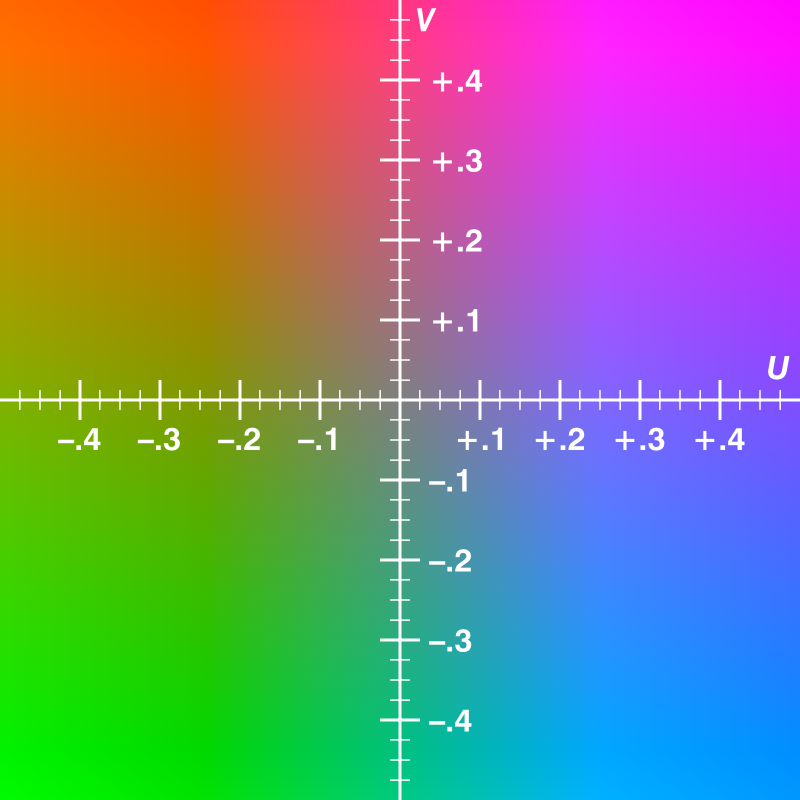
\includegraphics[width=0.5\linewidth]{images/UVPlane.png}    

    \caption{UV plane for the YUV encoding, notice how U is the green-blue axis and V is the red-yellow axis. Every RGB colour can be acquired by sampling from points on this plane.}

    \label{fig:uvplane} 
\end{figure}
We can simplify and further constrain the problem significantly by converting $X_{RGB}$ to a YUV encoding, $X_{YUV}$. Like RGB, the YUV model represents the image through 3 channels, the first channel Y encodes the brightness of the image while the other two channels U and V encode the image's green-blue and red-yellow projections (see figure \ref{fig:uvplane}). The benefit of this encoding is that the Y channel on its own is equivalent to a greyscale version of the image, this creates a dependency between the input $X_{YUV}$ and output $Y$ values, as the first channel of a YUV image will correspond to the greyscale conversion $Y$. The colour to greyscale conversion is then much simpler, as instead of multiplying $X_{RGB}$ by a coefficient matrix $A$ to acquire the greyscale output, we can simply multiply $X_{YUV}$ by a part diagonal matrix that isolates the $Y$ values.

We'll demonstrate this algebraically. The RGB to YUV conversion can be done by multiplying the $X_{RGB}$ by $C$, a matrix containing the coefficients to convert RGB pixels to YUV:
\begin{equation}
    C X_{RGB} = X_{YUV}.
\end{equation}
Substituting this into left side of the conversion we get:
\begin{equation}
    A C^{-1} X_{YUV} = Y.
\end{equation}
$A$ is kept on the left side and multiplied by $C^{-1}$, this results in the desired part diagonal matrix $\hat{I}$, that can isolate the Y values in $X_{YUV}$ to obtain only the greyscale value matrix $Y$:
\begin{equation}
    A C^{-1} = \hat{I}.
\end{equation}
Substituting this diagonal matrix into the left side of the equation we get the direct problem in YUV form:
\begin{equation}
    \hat{I} X_{YUV} = Y.
\end{equation}
With this more constrained reformulation of the problem, the approximate solution which will be solved in this project entails finding a colourisation function $f(Y)$ and a set of parameters $\theta$ that minimises the difference between the colourisation's YUV output $f_{\theta}(Y)$, and the UV ground truth $X_{YUV}$:
\begin{equation}
    \underset{\theta}{\operatorname{arg min}} |X_{YUV}-f_{\theta}(Y)|^2 \quad\;\; s.t. \; \hat{I} X_{YUV} = Y \quad \forall \; X_{YUV}, Y.
\end{equation}
% I think it is important to go on here and show that this makes the formulation much simpler.
% Now equation 3.7 is equivalent to just doing argmin |X_UV - g_theta (Y)|^2 and no constraint (I used g instead of f as technically it is a different function now).
% i.e. if you infer U and V, then I X_YUV = Y is satisfied by definition for any U and V.
We can further simplify the formalisation, due to the Y channel dependency between the input $X_{YUV}$ and output $Y$ values. The problem can now be solved more simply by finding a colourisation function $g(Y)$ that produces a UV output, and a set of parameters $\theta$ that minimises the difference between the function's output $g_{\theta}(Y)$, and the UV ground truth $X_{UV}$:
\begin{equation}
    \underset{\theta}{\operatorname{arg min}} |X_{UV}-g_{\theta}(Y)|^2.
\end{equation}

In this case the $\hat{I} X_{YUV} = Y$ constraint is satisfied by definition for any U and V.

\section{Deep Learning Methods}
\label{deeplearning}
Deep Learning (DL) is a subfield of ML which is also used to solve problems with difficult to define solutions. DL models allow us to tackle even more complex problems thanks to their greater ability to detect useful features in the data. As defined by Goodfellow, "DL models can learn from experience and understand the world in terms of a hierarchy of concepts, with each concept defined through its relation to simpler concepts"\cite{Goodfellow} (see figure \ref{fig:deeplearning}).
\begin{figure}[h]
    \centering
    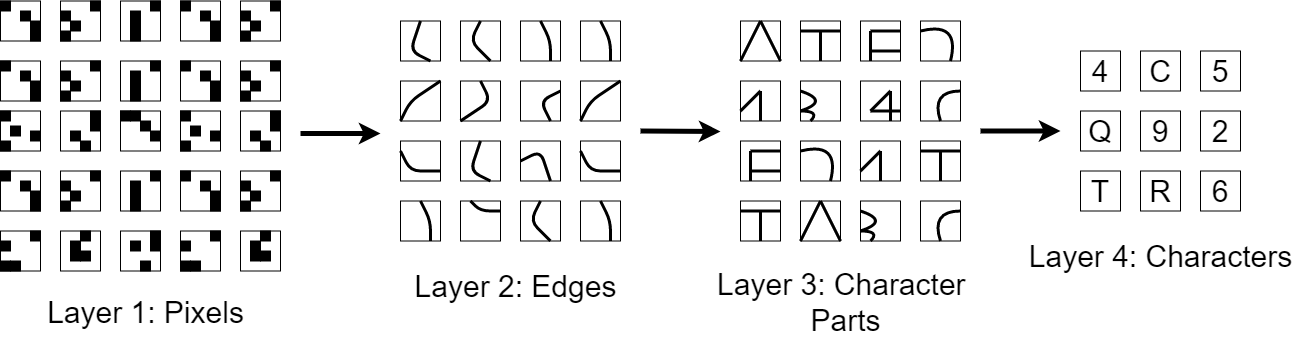
\includegraphics[width=1.0\linewidth]{images/DeepLearning.png}    

    \caption{Demonstration of how a Deep Learning model for character recognition would work: the model breaks the features of the character images into a hierarchy of abstraction. Lower layers analyse low level information like the individual pixels, then subsequent layers combine the information from previous layers to recognize, edges, parts, and eventually characters.}

    \label{fig:deeplearning} 
\end{figure}

The ability to extract hierarchies of features from data means DL is capable of finding useful feature priors in large amounts of image data, with relatively little tuning from the programmer compared to older ML models. This makes DL a good means with which to define an approximate solution to the problem of colourisation. The difficulty of manually defining a reliable set of priors to guide the colourisation process is solved as DL provides models which are very capable of automatically finding good priors and using them to guide the colourisation process. For an experimental demonstration of how feature recognition is employed by the models in this project to colourise images, see \ref{shapeseteval}.

\subsection{Neural Networks}
% https://towardsdatascience.com/activation-functions-and-its-types-which-is-better-a9a5310cc8f
% Neural-Networks are considered Universal Function Approximators. It means that they can compute and learn any function at all. Almost any process we can think of can be represented as a functional computation in Neural Networks
\label{nn}
Neural Networks (NNs) are the main systems involved in DL. They are powerful and scalable models which are capable of tackling highly complex ML tasks. The main component of a NN is a Neuron, which takes a set of numerical inputs ($X1, ... , Xn$) sometimes along with a bias value ($b$) and produces a numerical output ($Y$).

Inside the neuron, a weighted sum of its inputs is calculated:
\begin{equation}
    \Sigma = b + w1 * X1 + w2 * X2.
\end{equation}
Then an activation function is applied to this sum to constrain its result within a given range. There are a variety of different activation functions, however, for this example we will use the common ReLU function:
\begin{equation}\label{eq:sigma} 
    Y = max(0, \Sigma).
\end{equation}

\begin{figure}[h]
    \centering
    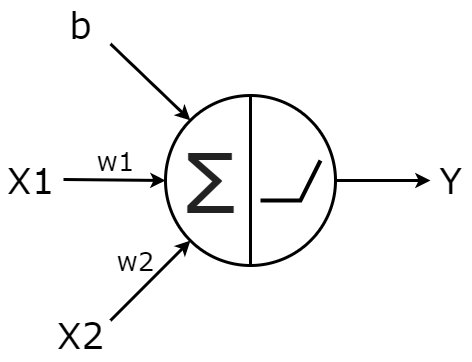
\includegraphics[width=0.4\linewidth]{images/Neuron.png}    

    \caption{The neuron calculates a weighted sum of its inputs (b, X1, X2), then applies an activation function (ReLU) to that sum and outputs the result (Y).}

    \label{fig:neuron} 
\end{figure}

In the case of a fully connected network, each neuron is connected to every other neuron in the previous and successive layers, receiving their inputs from them and propagating their outputs onward to others to eventually produce the expected result Y (see figure \ref{fig:neuralnet}). This inter-dependency of information between the layers is what allows NNs to model hierarchies of concepts as mentioned above, initial layers will be trained to extract useful information from low level details of the inputs which the next layer will then use to extract more relevant information from. 

The network trains itself by tuning the weights and biases (both referred to as "trainable parameters") for each neuron in order to produce an optimal output. The optimal output is found through the use of a loss function which calculates a value representing the difference between the expected output and the output given by the network for a particular input. The backpropagation algorithm is then used to adjust the parameters of each neuron by computing the gradient of the loss function with respect to the parameters for each input. The gradient indicates how the parameters need to be changed in order to reach a minima of the loss function. Reaching a minima means that the network is outputting something similar or equal to the expected output. 

\begin{figure}[h]
    \centering
    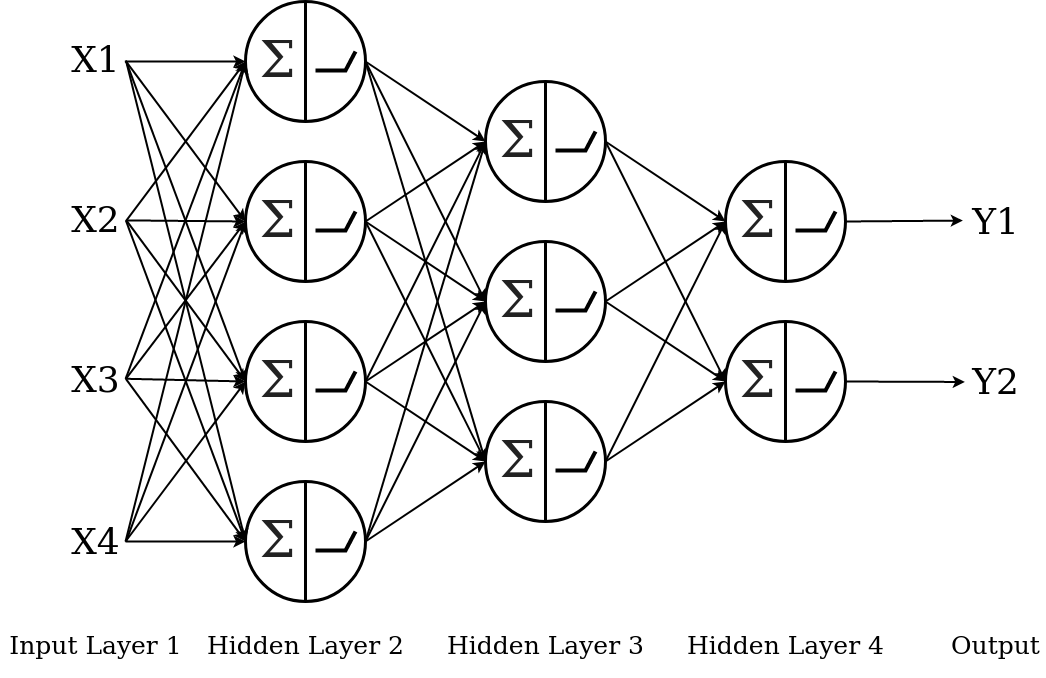
\includegraphics[width=1.0\linewidth]{images/NeuralNet.png}    

    \caption{Example of the dataflow structure of a NN. The number of X inputs, layers and Y outputs shown in this example are arbitrary and can vary in real NNs.}

    \label{fig:neuralnet} 
\end{figure}
%You need to explain backpropagation, and gradient descent

\subsection{Convolutional Neural Networks}
\label{convolution}
One Deep Learning system used in this project which is particularly effective in handling problems involving image analysis is the Convolutional Neural Network (CNN), these networks are able to extract specific patterns in images and learn how these patterns can combine into meaningful features.

The main element of the CNN is the convolutional layer which contains neurons capable of learning weights and biases for particular objects in an image. The first convolutional layers of a CNN are able to recognise low level features present in specific parts of the image, which can then be combined into higher level features for later layers to recognise. Unlike the fully connected layers of normal NNs, neurons in the first convolutional layer are only connected to particular pixels of the input image, then in successive layers, the neurons are only connected to particular neurons of the previous layer. These connections are made when the neurons or pixels of the previous layer or input fall within the range of a rectangular receptive field called the kernel. 

The kernel performs the convolution operation over subareas of the image within its range in order to produce a convolved output. The convolution consists of a matrix multiplication between the values in the portion of the image the kernel passes over and the weights of the kernel itself plus a bias (see figure \ref{fig:convolution}).

\begin{figure}[h]
    \centering
    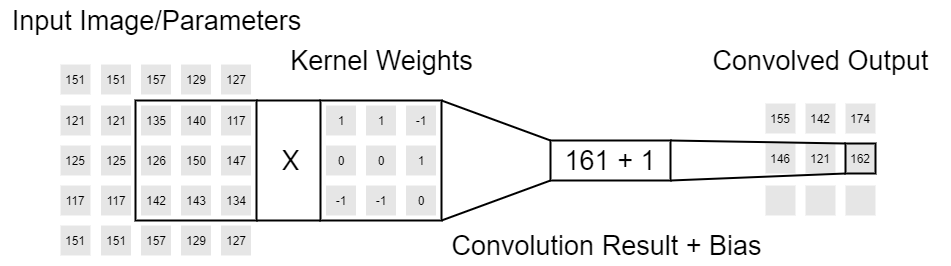
\includegraphics[width=1.0\linewidth]{images/Convolution.png}    

    \caption{Demonstration of a convolution, the kernel will eventually continue moving across the input matrix until it has convolved.}

    \label{fig:convolution} 
\end{figure}

% How do greater strides downsample the image??
The kernel will move over the entire image in strides, for instance 1 stride a turn means it will move along the image one pixel at a time, from left to right, top to bottom. Most convolutional layers have a stride greater than 1 that downsamples the size of the image with each convolution, this downsampling can isolate more important features of the image in the network, as portions which play a greater role in reducing the loss are more likely to be present in later layers after multiple downsamples. This process of downsampling also promotes "translational equivariance", which makes the model more tolerant to small translational changes in the input, i.e. making it easier for the model to notice an important feature in the image regardless of the feature's position. 

The size of the kernel is typically an odd dimension (often 3x3 or 5x5) as that allows it to visit particular pixels more than once as it convolves the image. This is useful as sometimes adjacent pixels may be part of features that are dependent on neighbouring pixels on different sides. For example, if a 2x2 kernel has a stride of 2, each stride will visit unique pixels meaning that it will not be able to model any kind of dependency between pixels in the different areas it visits. On the other hand, a 3x3 kernel with a stride of 2 will visit the same pixels on the edges of each area multiple times meaning that it can model a dependency between these pixels on the borders if it needs to.
% This last bit is messy, also efficiency might be another reason to downsample, you should talk about this technology in relation to the project itself
% Summarise why you use this

\subsection{Generative Adversarial Networks}
\label{gan}
Generative Adversarial Networks (GANs) are Deep Learning frameworks capable of generating data through an adversarial process. Two networks are trained in parallel, one being the generator and the other the discriminator. The generator generates new outputs from the training data while the discriminator calculates the probability that a sample came from the training data or is the output of the generator\cite{GANs}.

\begin{figure}[H]
    \centering
    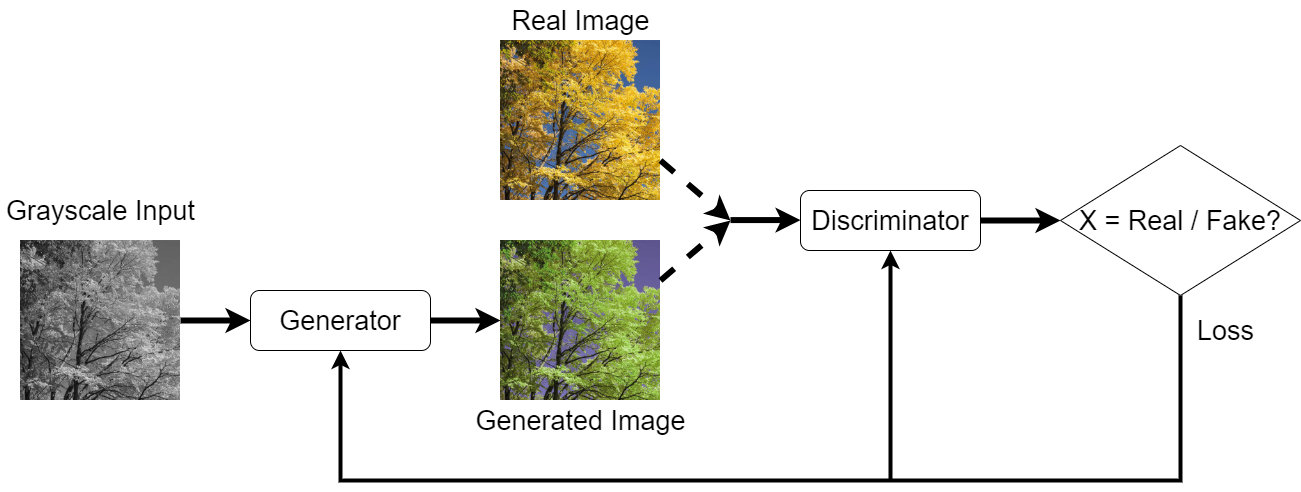
\includegraphics[width=1.0\linewidth]{images/GAN.png}    

    \caption{General structure of a GAN used for image colourisation.}

    \label{fig:gan} 
\end{figure}

Typically the generator network will be trained to generate candidates from a latent feature space. However for the purpose of image colourisation the generator is a CNN trained to produce colour images from greyscale inputs. The generator will train in order to maximise the probability of the discriminator classifying an image it produces as being a valid colour output. The discriminator is another CNN which maps a colour image to a single output probability representing the image's validity. This discriminator will initially be trained on the real images so it can recognise them, and thereafter will be further trained based on its ability to correctly validate images produced from the generator, attempting to minimise the probability of it making a mistake. Over time through training, the generator should produce better images while the discriminator will become more skilled at recognising generated images.

GANs are an effective method for providing generalised outputs due to the manner in which they are trained. Typical NNs are trained to produce a specific output for each given input, and thus have a tendency to "overfit". A model overfits when it is trained in a manner which conditions it too much to only recognise the data it has been trained on, and is then incapable of producing sufficient outputs for unseen data. When GANs train on the other hand, they use the adaptable output of another network, the discriminator, to determine whether what the generator is producing is valid. This process impedes it from overfitting to a specific dataset as much as a typical NN would due to the non-rigid state of the data it uses as a reference to train on. 

GANs are a very attractive method for modelling the process of image colourisation due to their ability to generalise better than typical NNs, allowing them to account for more of the important priors involved in colourisation, across a more diverse range of images. A downside to them however is the difficulty involved in training them, as they can be very sensitive to hyperparameter changes, and often the relationship between the generator and discriminator can be imbalanced and lead to overfitting. 
% https://medium.com/@jonathan_hui/gan-why-it-is-so-hard-to-train-generative-advisory-networks-819a86b3750b
% Should go back and change the format for introducing acronyms with the acronym in brackets after it's first mentioned (Variational Autoencoder (VAE))
\subsection{Variational Autoencoders}
\label{vae}
Variational Autoencoders (VAEs) are another form of Deep Generative model which generate data by sampling from a latent feature space. An encoder network is used to encode a given input to a compressed representation stored in the latent space Z, and then an encoder is used to decompress samples of this latent space in order to reconstruct equivalent outputs\cite{VAE}.

In standard Autoencoders (AEs) the latent space Z is a fixed vector. The larger this vector is, the greater the AE's ability to compress more details. The defining characteristic of VAEs, which sets them apart from AEs, is that the latent space is a distribution composed of a mean vector and standard deviation vector as opposed to a single fixed vector. With a fixed vector latent space, sampling from each entry of Z will always produce the same corresponding output Y, however with a distribution, latent space samplings can have a range of potential values within a respective standard deviation. In more formal terms, a VAE encodes an input X to a latent distribution $Q(Z|X)$, and decodes a sample from this distribution $P(X|Z)$ to produce an output.

VAEs are trained with a loss function composed of two terms. The first term is the reconstruction loss, which an AE would also use. This measures how effective the decoder has learned to reconstruct an input image by sampling from its latent representation. The second term of the loss is the KL divergence which learns how far removed the distribution is from a normal Gaussian, this tries to force the distribution to stay close to a mean of 0 and a standard deviation of 1. Due to the fact that backpropagation can't run through sampling nodes, VAEs sample from the latent space using a method known as the "Reparametrisation Trick". This trick takes a sample $z$ as the sum of a fixed mean $\mu$ plus a standard deviation $\sigma$, then multiplied by a value $\epsilon$ which is always a standard gaussian with mean 0 and standard deviation 1:
\begin{equation}\label{eq:reparametrisation_trick}
    z = \mu + \epsilon \sigma, \;\; \epsilon \sim \mathcal{N}(0,1).
\end{equation}
The $\mu$ and $\sigma$ are thus the only variables that need to be trained and which backpropagation needs to run through. 

For the task of image colourisation, the VAE needs a second conditional encoder which can take a greyscale image and produce a corresponding latent space representation that is equal or approximate to the colour image's latent representation (see figure \ref{fig:vaetrain}). During training, the training encoder is given a colour image $X_{YUV}$ and the conditional encoder is given the greyscale version of the same image  $X_{Y}$. The training encoder trains as normal to produce the latent space representation $Q(Z|X_{YUV})$, while the conditional encoder trains to replicate this same latent space for each greyscale encoding $Q(Z|X_{Y})$. After the network has been trained, the VAE uses the conditional encoder's latent distribution $Q(Z|X_{Y})$ in place of the training encoder's distribution $Q(Z|X_{YUV})$. A greyscale input can then be coloured by feeding it to the conditional encoder that produces a latent space mapping, which can then be fed to the decoder to produce a colourised output $P(X_{YUV}|Z)$ (see figure \ref{fig:vaetest}).

% Don't like this image
\begin{figure}[H]
    \centering
    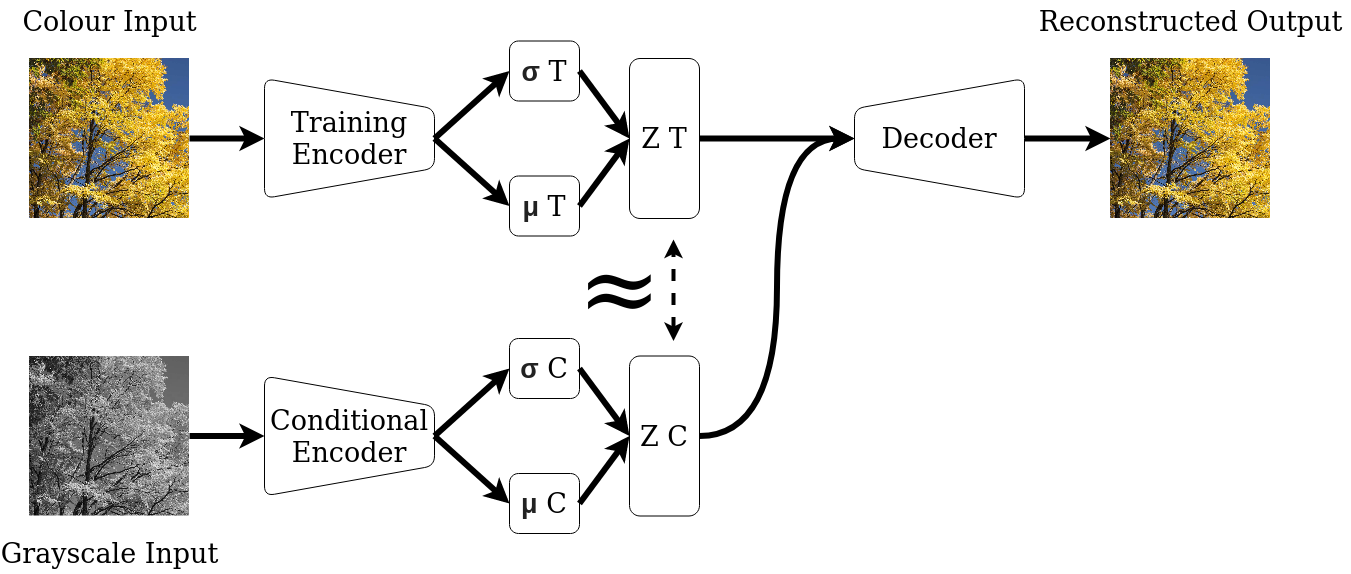
\includegraphics[width=1.0\linewidth]{images/VAETraining.png}    

    \caption{Structure of a colourisation VAE for training.}

    \label{fig:vaetrain} 
\end{figure}
\begin{figure}[H]
    \centering
    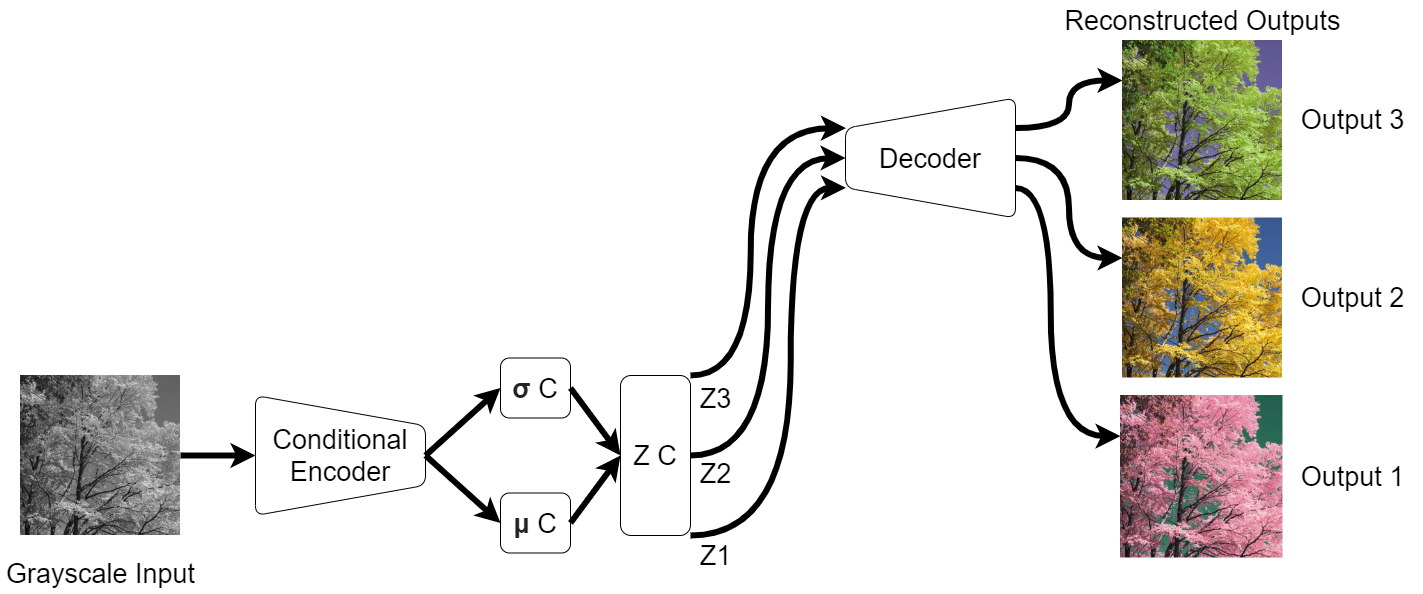
\includegraphics[width=1.0\linewidth]{images/VAETesting.png}    

    \caption{Demonstration of how a colourisation VAE uses the conditional encoder to provide a range of colourisations.}

    \label{fig:vaetest} 
\end{figure}

VAEs are an interesting tool for image colourisation as they are capable of modelling the diverse range of possible colourisations a greyscale image can feasibly correspond to. For each greyscale input, the VAE can map a range of potential latent representations with mean $\mu C$ and deviation $\sigma C$, each of which can then produce a different output when fed to the decoder. 

\section{Datasets}
Due to the complexity of the problem, the effectiveness of a model's ability to colourise is heavily dependent on the dataset it is trained on. Even very effective DL models can be useless if they aren't trained on datasets that are appropriate for the problem. A range of datasets were used to train and test with, each having their own benefits and disadvantages in terms of verifying the effectiveness of the model.

\subsection{Shape Set}
Shape Set is a small custom dataset made to test the network's ability to colourise images based on a clear symbol prior. Each image containing a shade of a particular colour inside a distinct corresponding shape. Blue colours are present inside circles, red colours inside squares, and green colours are present in triangles.
\begin{figure}[h]
    \centering
    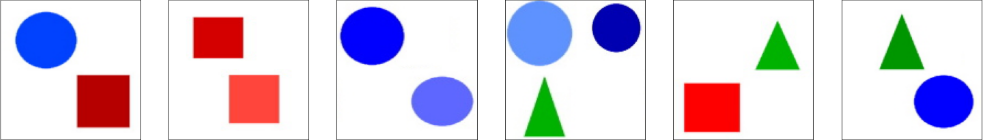
\includegraphics[width=1.0\linewidth]{images/ShapeSet.png}    

    \caption{Some sample images from Shape Set}

    \label{fig:shapeset} 
\end{figure}

\subsection{Cifar-10}
Cifar-10 is a widely used collection of 60'000 colour images spread equally amongst 10 different classes. Each image is 32x32 pixels large and thus the entire dataset is very compact at only 163MB. Due to its wide usage, the Keras library contains a simple to use function to conveniently download the dataset to the current workspace. Its small size and easy to use Keras setup made it an ideal dataset to quickly train models with, while also providing a large number of images with a great diversity of features which the network could train on. 

Its division into separate equally sized classes also allows the convenient selection of specific classes to train on. This limits the network to training with a more constrained set of images which have more features in common, helping it to better identify the most useful features for a given class. Training on a specific class is often a better way to evaluate a network, as datasets with too much diversity can make it difficult for any network to produce a satisfactory output. 

The low resolution of the images however makes it an insufficient dataset to train any kind of model that would be used in a realistic scenario, as such a resolution is so low that a lot of smaller features begin to be blurred and unnoticeable. A colourisation model intended for wider use would likely need to colour images with much more detailed features and thus would need to be trained on a higher resolution dataset where such features are more prominent and can be identified by the network.

\subsection{Faces}
Faces is a set of 750 cropped face images taken of people of different genders and ethnicities. The images are all of varying resolutions but for the purpose of training were resized to 128x128, this kept the image small enough to optimise training speed while at the same time keeping most of the main features clearly present in the image.

The people in these images are all facing different directions but generally towards the camera so that their face is clearly visible in each image. This means every image contains the same clear prior of a human face with the same facial features (nose, eyes, mouth, etc.). Training on this dataset is a good test to determine whether the network is capable of identifying a more complex set of symbolic priors than the ones contained in the symbol set in order to aid colourisation, and also serves as a demonstration of how constrained datasets of well categorised images can provide more reliable training results from most models.

The dataset is also a useful training set to evaluate models with after testing them with Cifar-10. The higher resolution of the images means the model has to train on a more complex dataset, however the important features that aid colourisation (facial features) are clearly present in every image. This makes the dataset a good in-between to test a model's ability to handle higher resolutions before presenting it with a challenging diverse dataset of more distinctive images.

\subsection{Imagenette}
Imagenette is a subset of 10 image classes taken from the ImageNet database. Each image is 160x160 pixels large but for the purpose of maximising training speed were resized to 128x128 as was the case for Faces. 

The classes of Imagenette are very disparate, with categories ranging from animals to buildings. This makes training on the entire dataset difficult. However, training on each class is a good way to measure how each model adapts to particular categories of images and which categories present more of a challenge to each model. 

The dataset is also very noisy as can be seen in figure \ref{fig:imagenette}. The main object of the image varies greatly in terms of orientation, lighting, and size. This makes the dataset very challenging for most networks, even when it's only looking at a particular category, as identifying the important features that can aid colourisation is made much more difficult by the noise and variation of the images.

\begin{figure}
    \centering
    \begin{subfigure}[b]{1.0\textwidth}
        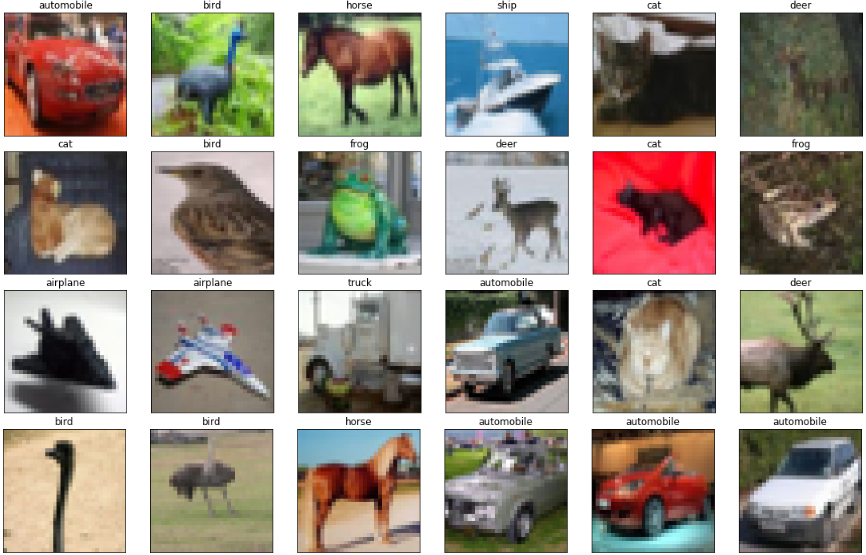
\includegraphics[width=\textwidth]{images/cifar10.PNG}
        \caption{Sample images from Cifar-10 with corresponding classes above.}
        \label{fig:cifar10}
        \vspace*{5mm}
    \end{subfigure}
    \begin{subfigure}[b]{1.0\textwidth}
        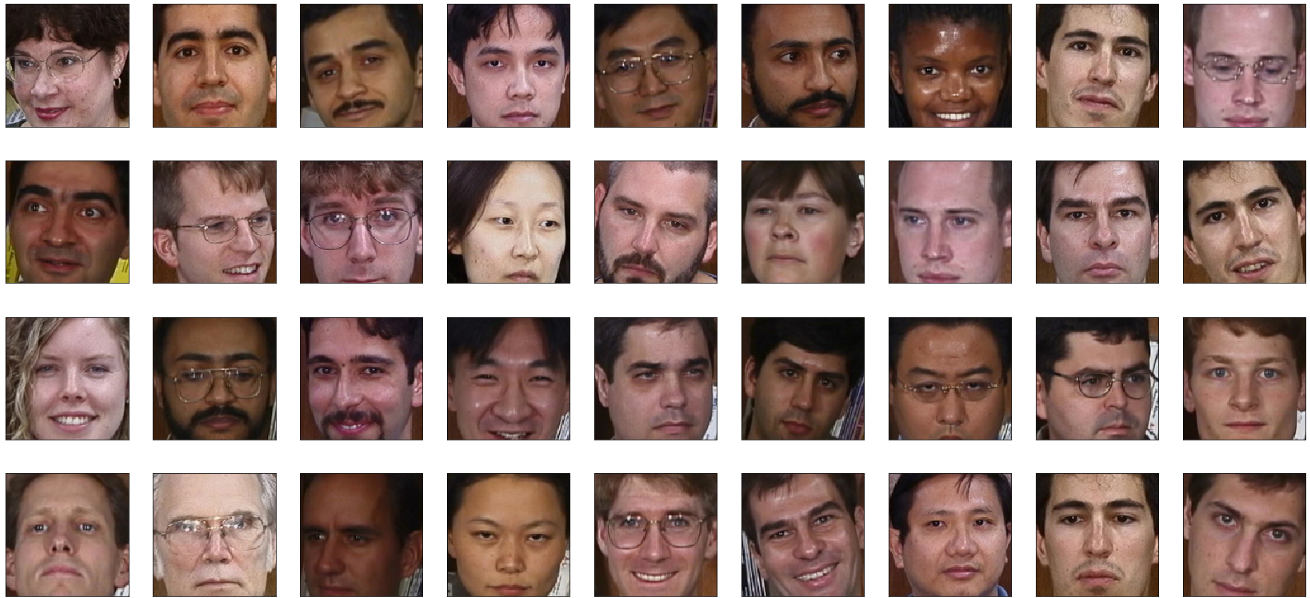
\includegraphics[width=\textwidth]{images/celeb_faces.PNG}
        \caption{Sample images from Faces.}
        \label{fig:celebfaces}
        \vspace*{5mm}
    \end{subfigure}
    \begin{subfigure}[b]{1.0\textwidth}
        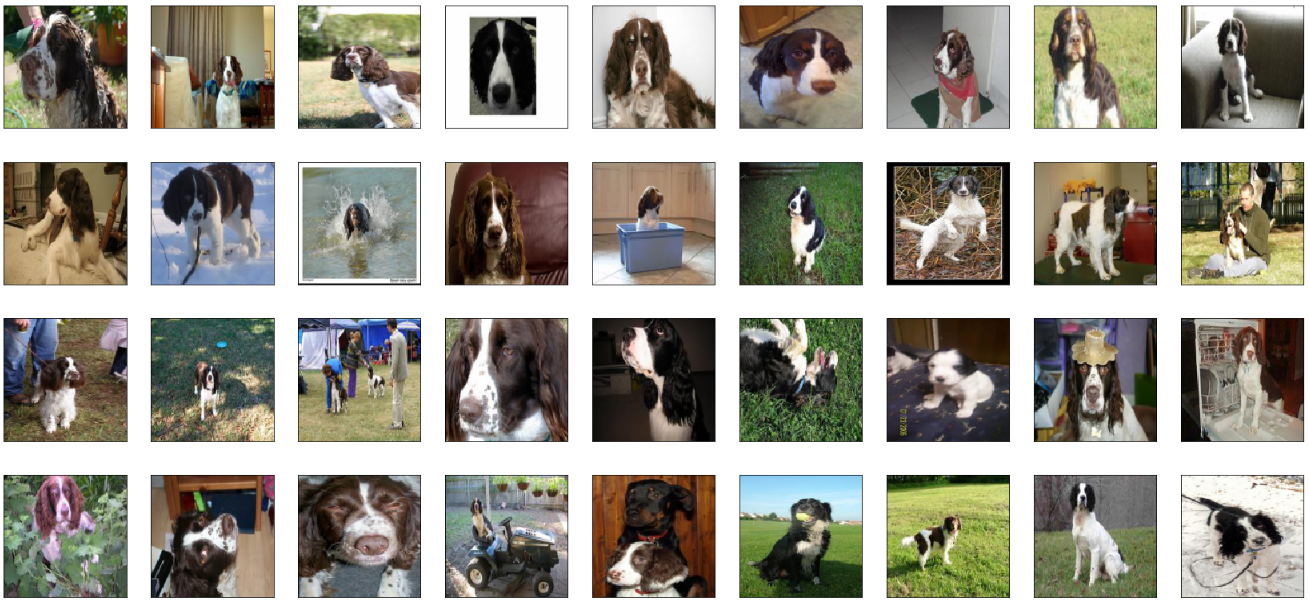
\includegraphics[width=\textwidth]{images/imagenette.PNG}
        \caption{Sample images of the Dog category from Imagenette.}
        \label{fig:imagenette}
    \end{subfigure}
    \label{fig:datasets}
\end{figure}

% Keras section?
% Could only use Keras compatible techniques

\section{Google Colab}
% Could go into more detail about how it's so convenient
Google Colab is a free, browser-based, Python notebook environment that allows the user to run their code on Google's own cloud hardware. Each model developed for this project was written, trained, and evaluated using Colab as it provided a convenient and free platform on which to develop and run Machine Learning code. 

Because Colab is browser-based, each notebook written on it is conveniently accessible from any machine. The notebooks themselves are saved on the user's Google Drive account, and the user is also able to use their Drive to save and load data from within the notebook's code. This Drive integration provided a useful platform on which to host datasets, as well as a space to save and load trained models.

Code run on Colab can use Google's own GPU and TPU hardware accelerators, making it a good platform for NN training which involves a great number of tensor operations that can be carried out faster with such hardware. Code containing training loops can be conveniently run in the background, however a maximum of only two notebooks can be run at any point in time. Notebooks can also only run so long as a browser created session is still running, so closing the browser which a notebook is currently running on will end the training loop. These limitations made it difficult to train models with large datasets or a large number of parameters as the browser needed to be kept open for extensive periods of time.

%==================================================================================================================================
\chapter{Implementation}
In this chapter we will explain the designs of each model and the reasoning behind their design choices.

\section{Convolutional Neural Network}
\label{cnn-implementation}
% Could even talk about how this relates to related work
The first model which was developed was a Convolutional Neural Network (CNN), which is a Neural Network (explained in \ref{nn}) made using convolutional layers (explained in \ref{convolution}). This was a deterministic model capable of producing a single corresponding colourisation for each unique greyscale input. This network was developed first as it was the simplest viable DL solution, and because it could then be reused as part of the later generative models after a suitable design for it was found.

As explained in \ref{yuv-encoding}, the colourisation model needs to take a 3-dimensional tensor as input, representing a greyscale image in the form of the Y channel of a YUV image, the model must then find an algorithm to produce the corresponding U and V colour channels of that YUV image. This means that the input to the network will be a rank 3 tensor of the shape (Shape: Width, Height, 1) and the output will be (Shape: Width, Height, 2).

\subsection{Architecture}
Typically when implementing ML algorithms, a range of candidate parameters are chosen and then an exhaustive search is performed over each subset in order to find the optimal configuration that optimises the model. When designing Neural Networks this approach isn't feasible due to the large amount of parameters involved as well as the long periods of time necessary to train most models that Colab can't support. Designing a model ultimately had to be done through trial and error, repeatedly testing and tuning models in order to finally find a model with the best performance that overfits or underfits the least.

Models overfit or underfit based on their "capacity" meaning their ability to fit a wide variety of functions. Low capacity models can underfit the dataset as they lack the capacity to memorise important information, while high capacity models can overfit by memorising too many properties of the training data that won't help their performance on unseen data\cite[p.110]{Goodfellow}. The primary parts of a CNN which govern its capacity are the number of hidden layers it has, the number of filters present in these layers, and the kernel size and strides for each layer which determine the downsampling (explained in \ref{convolution}). These main elements were the most important parts of the CNN that needed to be decided through repeated testing before other parameters could be determined.

Along with the general structure of the network, there were some important parameters that also needed to be decided before the model could be trained. A loss function first needed to be chosen to indicate the error between the output of the network and the ground truth. The task the network had to perform can be seen as a form of regression, where it estimates the relationship between an image's greyscale features and a colour encoding, and for most regression problems the  Mean Squared Error (MSE) is the most commonly used loss function. MSE calculates the loss as the mean of the squared sum of the differences between $n$ output values $y'$ and $n$ expected values $y$: 
\begin{equation}
    MSE = \frac{1}{n}(\sum_{i=1}^{n} (y_i - y'_i)^2).
\end{equation}
Another popular regression loss function was Mean Absolute Error, which is a similar formula however takes the absolute difference of the sum of output and expected values as opposed to the squared root. MAE wasn't used as it penalises larger errors less than MSE does, leading to less precise output values.

Activation functions needed to be chosen for each hidden layer along with a precision activation for the output layer. Using computationally expensive activations in the hidden layers would slow training considerably for diminishing improvements on performance, a more complex activation on the output layer however is affordable as the precision of the final result matters more than the accuracy of the many feature activations. ReLU functions (explained in \ref{eq:sigma}) were chosen for the inner layers of the network as they were the simplest and thus the quickest for the network to calculate. For the output layer, tanh functions were chosen which are defined as:
\begin{figure}[h]
    \centering
    \begin{subfigure}[b]{0.4\textwidth}
        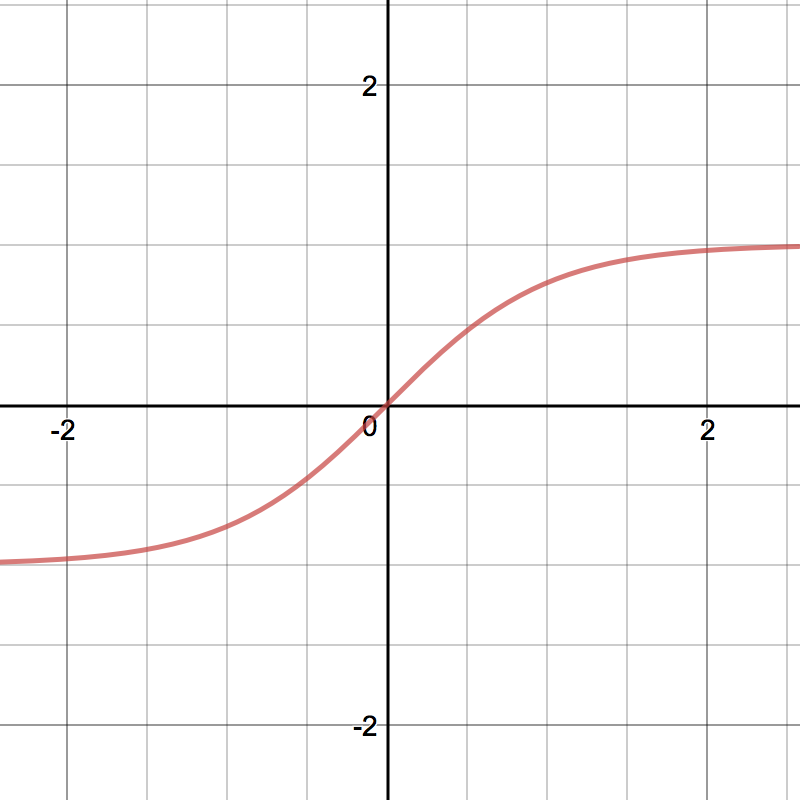
\includegraphics[width=\textwidth]{images/tanh.PNG}
        \caption{$tanh(x) = \frac{2}{1+e^{-2x}}-1$}
    \end{subfigure}
    \quad
    \begin{subfigure}[b]{0.4\textwidth}
        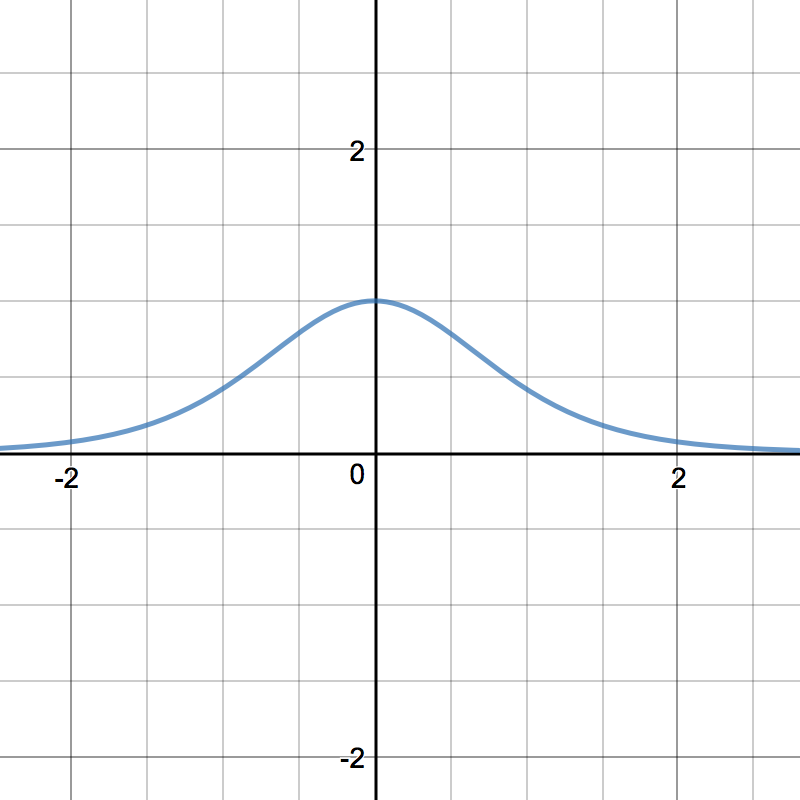
\includegraphics[width=\textwidth]{images/tanh_prime.png}
        \caption{$tanh'(x) = 1 - tanh(x)^2$}
    \end{subfigure} 
\end{figure}

Tanh functions have steep derivatives that help the network minimise its contribution to the loss relatively quickly. This is because the backpropagation algorithm adjusts the network's weights in the direction of the steepest descent surface defined by the total error observed, so larger derivatives correspond to more significant weight updates.

% activation functions with large derivatives give more information to the backpropagation algorithm, allowing it to apply more significant updates at each step of training. Weights are adjusted in the direction of steepest descent surface defined by the total error observed
% https://ml-cheatsheet.readthedocs.io/en/latest/activation_functions.html
% Should try to explain this better

An optimiser also needed to be chosen, which refers to a function used to find minima of the loss function. As a preliminary optimiser, Stochastic Gradient Descent (SGD) was used, as it is the most basic optimiser and could be used as a good baseline from which to measure the performance of other optimisers when parameter tuning later on.

To design the network, two models were initially chosen, one very shallow model with a small number of layers and filters (see figure \ref{fig:shallow_model}) and a contrasting very deep model with a large number of layers and filters (see figure \ref{fig:deep_model}). The models were both trained on the same data and the output of the loss over training was plotted in order to determine how far each model was from a well fitting design. 

% If you have time you should re run these experiments with smoothed loss functions
\begin{figure}[h]
    \centering
    \begin{subfigure}[b]{0.5\textwidth}
        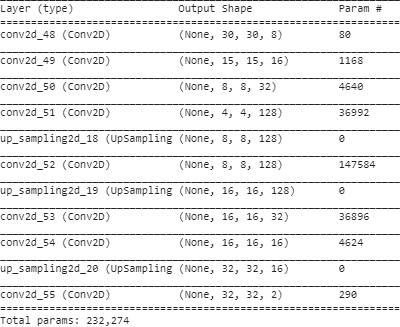
\includegraphics[width=\textwidth]{images/FinalBasicModel.PNG}
        \caption{}
    \end{subfigure}
    \quad
    \begin{subfigure}[b]{0.41\textwidth}
        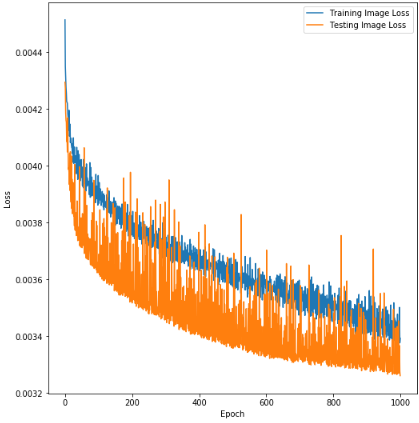
\includegraphics[width=\textwidth]{images/FinalBasicModelLoss.PNG}
        \caption{}
    \end{subfigure} 
    \caption{Final basic model with accompanying loss. Notice how the training and testing loss are continuing to descend, with enough epochs the training loss will go below the validation loss however the important thing is that both the losses continuously descend together. This means that the network has just enough capacity to store the most important information necessary for the problem that can help it generalise without overfitting.}
    \label{fig:final_basic_model}
\end{figure}

After repeating the two model method with an increasingly shallow deep model and an increasingly deep shallow model, an in-between model was eventually found that achieved the best loss output for both the training and testing dataset (see figure \ref{fig:final_basic_model}). With the basic structure decided, the next step was tuning the higher level parameters. 

\subsection{Hyper-Parameter Tuning}
% Do I need to explain that I used Keras?
Unlike the structure of the neural network, the hyper-parameters can feasibly be tested using an exhaustive search. Unfortunately however, the available libraries (Hyperas and ScikitLearn) that could do this for Keras models were both incompatible with Google Colab, so hyperparameters also had to be chosen through trial and error.

The first hyper-parameter that had to be chosen was batch size, which is the number of samples the network loads and trains on at each iteration. This value was conditioned mostly by the amount of RAM available on Google Colab, as even a relatively low memory dataset like Cifar-10 could exhaust Colab's available RAM when trained on a large enough network. The batch size thus needed to be at most 5,000 in order to train most models. The choice of batch size also has a significant impact on model learning; lower batch sizes result in less accurate updates, as the model will calculate gradients based on the batch it's currently working on which often isn't representative of the wider training dataset. This impact that low batch sizes can have results in a more stochastic training process and in some situations can be beneficial if the network can get stuck in local optima or overfit easily. Small batch sizes however can significantly slow down training, as more batches need to be transferred from storage to RAM in order to feed to the model. 

\begin{table}[h]
    \centering
    \caption{}
    \label{tab:operators}
    \begin{tabular}{lll}
        \textbf{Batch Size} &   \textbf{Final Loss after 100 Epochs}      &   \textbf{Training Time}  \\    
        \texttt{1024}           &   \texttt{0.0039}                     &   \texttt{2 min 27 sec}    \\
        \texttt{512}            &   \texttt{0.0038}                     &   \texttt{2 min 32 sec}   \\ 
        \texttt{128}            &   \texttt{0.0036}                     &   \texttt{3 min 43 sec}   \\
        \texttt{32}             &   \texttt{0.0035}                     &   \texttt{5 min 30 sec}   \\
        \texttt{16}             &   \texttt{0.0034}                     &   \texttt{7 min 6 sec}    \\
    \end{tabular}
\end{table}

Although lower batch sizes lead to a better loss value after the same amount of epochs, the time required to train on lower sizes got significantly higher for diminishing improvements on the final loss. The final batch size that was chosen was 512, as it provided a more fair balance between training time and performance.

A better optimiser also needed to be chosen, and there were two which both seemed like good potential candidates: RMSProp, and Adam. Both of these are popular extensions to the classic SGD and can often achieve better results. An important parameter that needed to be tested alongside the optimiser was the learning rate. Different optimisers can have very different performances based on their learning rates and so these two things needed to be tested together for a more reliable comparison. The learning rate dictates how much the model changes its parameters at each iteration in order to minimise the loss. Larger learning rates train faster, but can result in the model converging too quickly and overfitting before being capable of accounting for the less evident features that can help it generalise. If the learning rate is too small though it can result in the loss plateauing early as it may be incapable of making significant changes to the model. A general range of different rates were tested on the network for each optimiser (see figure\ref{fig:learning_rates}) and the most successful configuration proved to be Adam with a learning rate of 0.001. It made sense that Adam proved so effective as it is commonly employed for Computer Vision tasks\cite{Adam}. This is likely due to the fact that Adam is particularly effective for problems with "noisy gradients", meaning the network's parameters can still be tuned effectively even if the tuning information given by the backpropagation algorithm can vary greatly as it can for this problem. 

\begin{figure}[H]
    \centering
    \begin{subfigure}[t]{0.48\textwidth}
        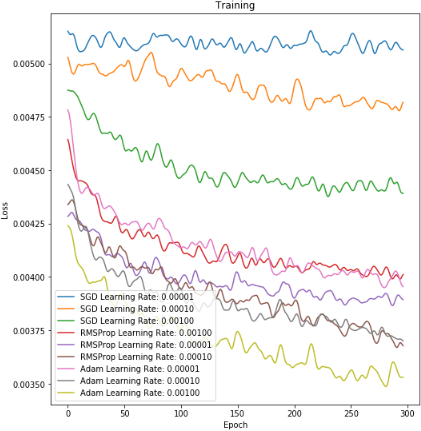
\includegraphics[width=\textwidth]{images/OptimiserComparison.png}
        \caption{Effect of different learning rates and optimisers on training the DCNN. The optimiser that achieved the best results was Adam with a learning rate of 0.001.}
        \label{fig:learning_rates}
    \end{subfigure}
    \quad
    \begin{subfigure}[t]{0.48\textwidth}
        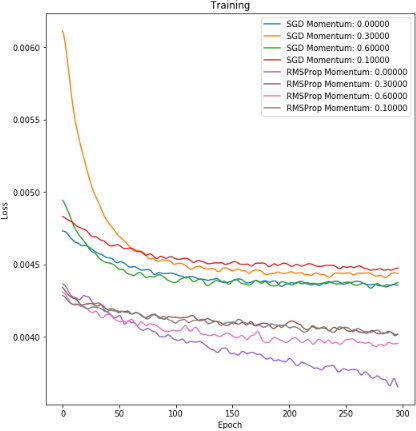
\includegraphics[width=\textwidth]{images/MomentumComparison.png}
        \caption{Effect of different momentum values and optimisers on training the DCNN. Momentum doesn't seem to provide any noticeable benefit for training with any of the optimisers.}
        \label{fig:momentum}
    \end{subfigure} 
    \caption{}
    \label{fig:hyperparameters}
\end{figure}

Although Adam seemed to be the best optimiser, RMSProp has a particular hyper-parameter called "momentum" which in some cases can be very effective at improving model performance. Momentum helps prevent the network getting stuck in local minima by also recording the direction its gradients previously moved towards. Higher momentum means that steps will follow a direction which is closer to the direction the previous step took. Tests were also run to determine if RMSProp with momentum could outperform Adam (see figure \ref{fig:momentum}), however any amount of momentum greater than 0 only worsened training. This is likely because of the high dimensionality of the data, as there would probably be a large variation in the ways the gradient could move in order to decrease the loss. Constraining it to a more fixed direction thus only prevented it from moving in the correct direction.

\subsection{Data Augmentation}
% More augmentation requires more training
Data augmentation was used to help prevent the model from overfitting by expanding the training dataset with slightly modified versions of the original images. This technique helps the model as the modified images will still contain the same important features however will be altered in such a way that the network has the opportunity to recognise them presented in another manner, promoting translational equivariance (explained in \ref{convolution}). The choice of how this data is augmented is important as it can also contribute to overfitting if not done correctly. If the modifications don't change the image significantly enough then the network will be exposed to a very similar image multiple times. 

The data augmentation techniques that were tested for training were:
\begin{enumerate}
    \item Horizontal flipping: the columns of each image were reversed.
    \item Rotation: each image was randomly rotated within a range of 60 degrees.
    \item Width and Height shifting: the pixels of each image were moved either horizontally or vertically by 20\%.
    \item Brightness: images were randomly darkened or brightened within a 50\%-150\% range.
    \item Zooming: randomly zooms in or out on images within a 50\%-150\% range.
\end{enumerate}

These different techniques were tested individually to see what impact they had on the model's performance (see figure \ref{fig:augmentation_testing}), and after the best augmentation techniques were found they were tested together to find which combinations worked best (see figure \ref{fig:augmentation_futher_testing}). In the end, Horizontal Flipping, Width and Height shifting, and Rotation were used to augment the dataset used by the CNN. These forms of augmentation had a significant impact on improving the model's ability to generalise (see figure \ref{fig:augmentation}).

\begin{figure}[H]
    \centering
    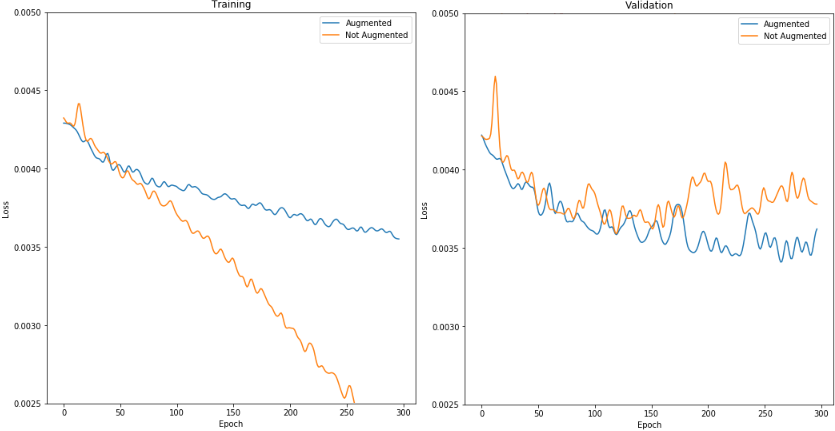
\includegraphics[width=0.9\linewidth]{images/Augmentation.PNG}    

    \caption{Effect of data augmentation on training and validation loss. Augmentation results in the validation loss much more closely approximating the training loss, meaning that the model is generalising better with it.}

    \label{fig:augmentation} 
\end{figure}

\subsection{Regularisation}
% https://towardsdatascience.com/l1-and-l2-regularization-methods-ce25e7fc831c
% https://towardsdatascience.com/intuitions-on-l1-and-l2-regularisation-235f2db4c261#f810
One final technique used to encourage the model to generalise was regularisation, which refers to a set of techniques used to constrain the network to learning sparse features, preventing it from simply memorising specific details of the training dataset. 

The first regularisation technique that was tried was L1 and L2 regularisation. Both of these methods work by adding an extra penalty term to the loss function to prevent large weight changes in the model, this penalty term being the norm of the model's weight vector (regularisation for the model's biases also exists however its impact on training was small). These forms of weight regularisation are named after the particular norm with which they're calculated. 

The L1 norm is defined as the sum of the magnitudes of the weights:
\begin{equation}
    ||w||_{1} = |w_{1}| + |w_{2}| + ... + |w_{N}|.
\end{equation}

The main attraction to L1 regression is that it shrinks the less important feature’s coefficient to zero, removing some features altogether. This works well for feature selection like colourisation as we have a huge number of features to consider with some that may not aid the colourisation process at all.
\begin{figure}[H]
    \centering
    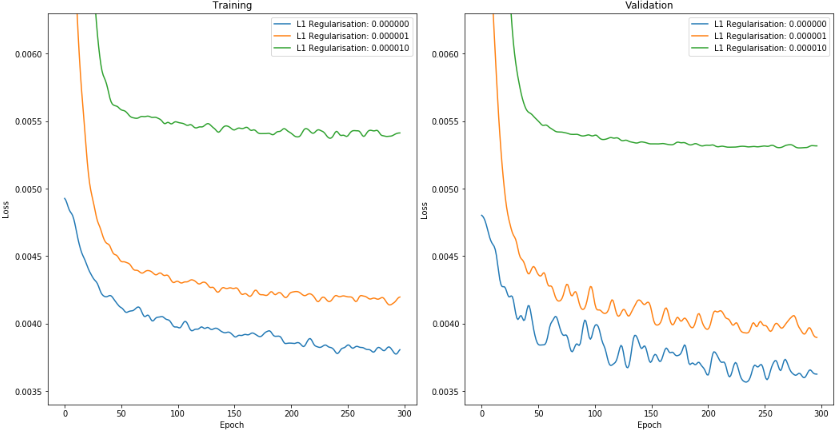
\includegraphics[width=0.9\linewidth]{images/L1Regularisation.PNG}    

    \caption{Training and Validation loss of various L1 regularisation values on the CNN. Any amount of L1 regularisation only appeared to worsen the both the training and validation loss.}

    \label{fig:l1regularisation} 
\end{figure}

The L2 norm is defined as the square root of the sum of the square weights:
\begin{equation}
    ||w||_{2} = (|w^2_{1}| + |w^2_{2}| + ... + |w^2_{N}|)^{1/2}.
\end{equation}
L2 regression is less severe, as it never decreases any of the features to 0 (although some can come very close), this is ideal in situations where there is always some level of dependency between the features which should be accounted for. To be certain that either could improve the model's performance they were both tested. 
\begin{figure}[H]
    \centering
    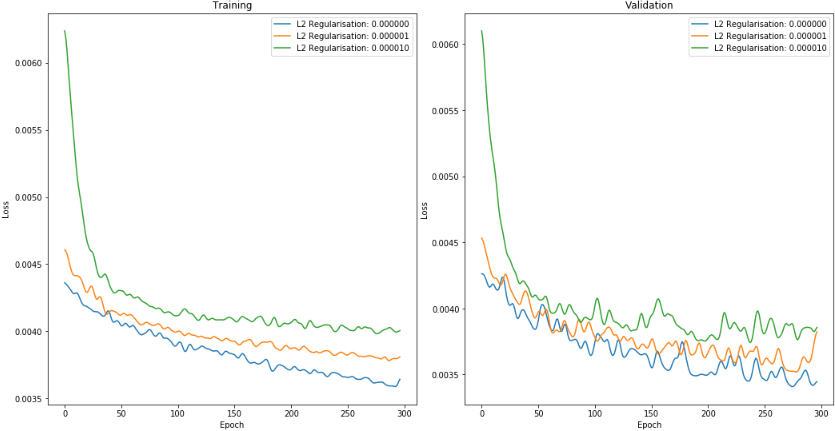
\includegraphics[width=0.9\linewidth]{images/L2Regularisation.PNG}    

    \caption{Training and Validation loss of various L2 regularisation values on the CNN. Just like L1 regularisation, L2 regularisation only worsened the performance of the model.}

    \label{fig:l2regularisation} 
\end{figure}

Another regularisation method was Dropout, which entails excluding random sets of neurons from each iteration of the training process based on a given probability. This can be very effective at reducing overfitting because it prevents neurons from becoming overly dependent on other neurons in previous layers, thus helping them recognise more general features by forcing them to consider information from the neurons that weren't excluded. A reasonable range of dropout values were tested (see figure \ref{fig:dropout}) and a final small dropout value of 0.2 was used.
\begin{figure}[H]
    \centering
    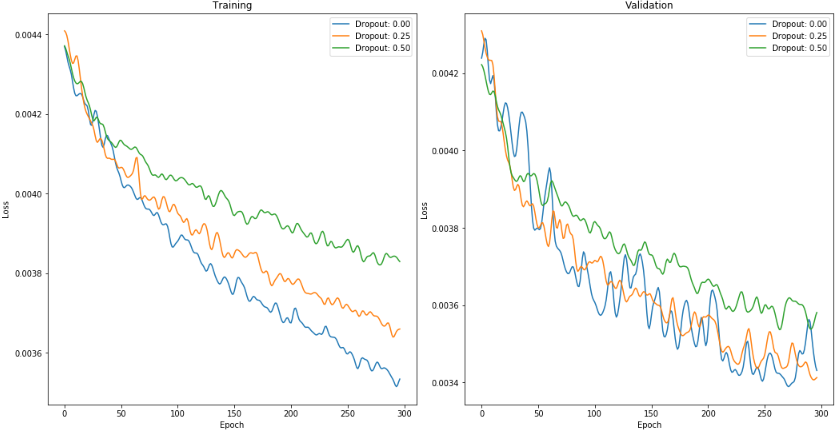
\includegraphics[width=0.9\linewidth]{images/Dropout.png}    

    \caption{Training and Validation loss of various Dropout probabilities on the CNN. Higher dropout values caused the training loss to plateau earlier however the middle dropout value of 0.25 did seem to have a small noticeable improvement on the stability of the validation loss.}

    \label{fig:dropout} 
\end{figure}

\section{Convolutional Generative Adversarial Network}
\label{gan-implementation}
% https://machinelearningmastery.com/how-to-develop-a-generative-adversarial-network-for-a-cifar-10-small-object-photographs-from-scratch/
% https://machinelearningmastery.com/impressive-applications-of-generative-adversarial-networks/
After an adequate CNN design was found, it could then be used as the base model for the generator of the Convolutional Generative Adversarial Network (CGAN). The CGAN is an implementation of the GAN (explained in \ref{gan}) designed to solve computer vision problems through the use of convolutional layers. It was the first generative model that was implemented due to the fact that its relatively widespread use for the task of image colourisation and so there were a substantial number of reference projects available that could be consulted in order to support our own implementation.

Like the CNN, the CGAN needs to take a 3-dimensional tensor as input, containing the Y channel of a YUV image, and is trained to model general mappings for U and V colour channels of that YUV image. It thus has the same input and output shapes as the CNN.

The trial and error process of designing the model used for the CNN couldn't be relied on when deciding the structure and parameters of the CGAN, due to the considerably longer amount of time needed to train it. Many of the design choices thus had to be made using suggestions and based on previously used methods that were successful in other projects. The relatively long amount of timed required to train the CGAN is demonstrated in \ref{computationtime}.

\subsection{Discriminator}
The first step was to design a discriminator that could accurately validate an image as being real or generated. The discriminator model takes as input a 3D tensor containing the U and V channels of a YUV image, and outputs a prediction between 1 and 0 representing the degree of belief for whether the image is real or fake. It was implemented as a CNN, but unlike the generator, it convolves from the UV tensor to a single value output as opposed to convolving from a Y tensor to a UV tensor. 

% https://towardsdatascience.com/gan-ways-to-improve-gan-performance-acf37f9f59b
The most important thing that had to be considered when designing the capacity of the discriminator was that it should only be effective in proportion to the generator, if the discriminator is too good then its outputs will be close to the two extremes of either 1 or 0 and the generator will struggle to tune itself proportionate to the error it's making. On the other hand, if the discriminator isn't accurate enough, its evaluations can be unreliable and it could mislead the generator to producing poor outputs. The discriminator was made to be of a higher capacity than the generator so it could give quality information without being too accurate. 

With regards to the loss function, the task the discriminator had to perform can be seen as a form of classification, as it classifies an image as being real or fake. For most classification tasks, Cross-Entropy is used, and as this only had to perform a binary classification, a more specific Binary Cross-Entropy (BCE) loss function could be used. BCE can be defined with the following equation, where $y$ is a binary value representing the correct prediction, and $p$ is the prediction probability:
\begin{equation}
    BCE = -{(y\log(p) + (1 - y)\log(1 - p))}
\end{equation}

Like the CNN, Adam was chosen as the optimiser for the discriminator. This is because the same computer vision challenges which Adam helps the CNN with also apply to the discriminator, as both networks rely on feature extraction to produce optimal outputs. 

For the activation functions, ReLU's were also used for the hidden layers for the same reasons they were used in the CNN, but for the output a Sigmoid function was used. The sigmoid function is defined as:
\begin{figure}[H]
    \centering
    \begin{subfigure}[b]{0.4\textwidth}
        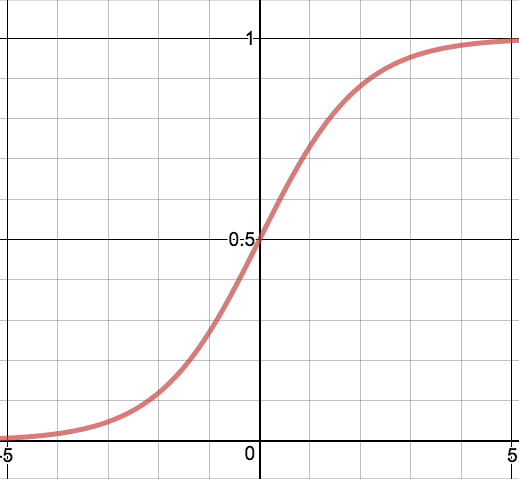
\includegraphics[width=\textwidth]{images/sigmoid.png}
        \caption{$sig(x) = \frac{1}{1+e^{-x}}$}
    \end{subfigure}
    \quad
    \begin{subfigure}[b]{0.4\textwidth}
        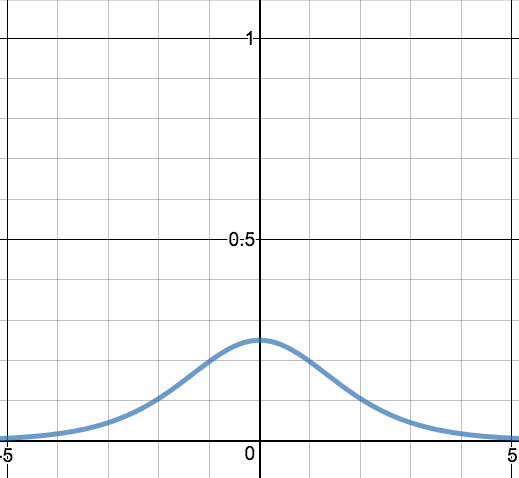
\includegraphics[width=\textwidth]{images/sigmoid_prime.png}
        \caption{$sig'(x) = sig(x)(1-sig(x))$} 
    \end{subfigure} 
\end{figure}

Although the sigmoid's gradients aren't as sharp as tanh's, its outputs are bound to a 0-1 range which is ideal for providing the binary classification output.

\subsection{Generator}
While the CNN we already designed served as a good base model for the CGAN's generator, some alterations had to be made in order for it to be viable as a generator.

Batch normalisation was added at particular points in between convolutional layers, which standardises the input of each layer so that it has a mean of 0 and a standard deviation of 1. This means that very diverse images can be made part of a closer distribution which the network can work with more easily, helping it generalise better. Batch normalisation is strongly recommended by \cite{DCGAN}, as it stabilises learning and helps deal with training problems due to poor initialisation, helping gradients to flow. Batch normalisation was only applied to most of the layers after the input and before the output layer, as applying it to every layer lead to instability.

The generator was also compiled without a loss function. This is because the generator isn't trained based on its own performance, but on the performance of the discriminator. More updates are made to the generator when the discriminator is giving correct evaluations, and less updates are made otherwise. The loss of the generator is given by the loss of the combined model which is explained in the next section.

Dropout was also removed from the generator. While in the case of the CNN it aided generalisation, for the CGAN it only added a further handicap to the generator, making it less capable of producing outputs which the discriminator would consider real. The general adversarial method which a CGAN trains with should be enough to aid the model's ability to generalise on its own, so regularisation methods like dropout are no longer necessary.

\subsection{Combined Model}
The final CGAN model was implemented by stacking the generator and discriminator networks into a combined model that allowed them to train together. Within the model, the generator can generate samples that are then passed as inputs to the discriminator, then the outputs of the discriminator are then used to indicate the loss of the generator in order to update it. 

For each training step, the discriminator is trained first, then the generator is trained after. The discriminator trains on a batch of the UV tensors from the training dataset based on the expected output of them being classified as real, then it trains on the batch of UV tensors produced by the generator based on the expected output that they're fake. The discriminator's total loss is subsequently calculated as the sum of the BCE losses returned from training on the real and fake batches. The generator is then trained after as part of the combined model and the loss is calculated as the BCE loss between the generated images being evaluated as real and the discriminator's own evaluation. I.e. the $y$ term of the BCE is that each generated output is real and the $p$ term is what the discriminator actually evaluated the output as.

\begin{figure}[H]
    \centering
    \begin{subfigure}[b]{0.48\textwidth}
        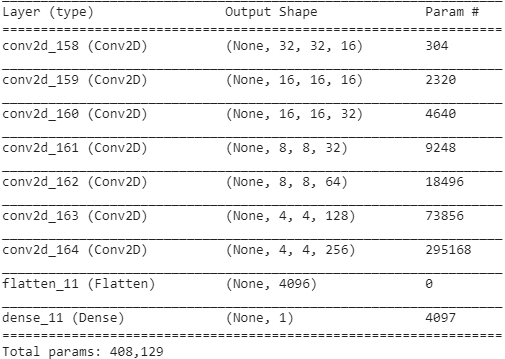
\includegraphics[width=\textwidth]{images/Discriminator.PNG}
        \caption{Final discriminator structure.}
    \end{subfigure}
    \quad
    \begin{subfigure}[b]{0.48\textwidth}
        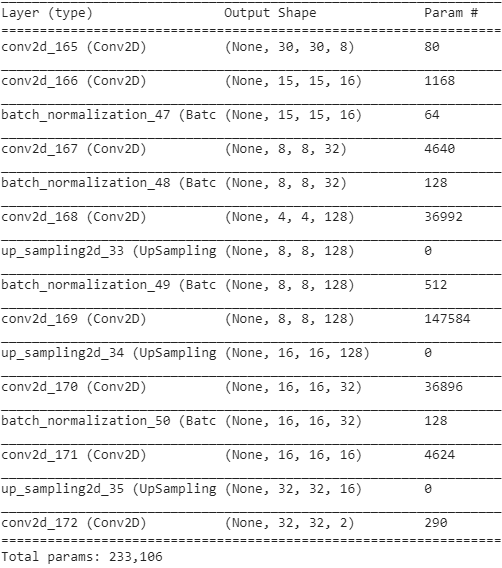
\includegraphics[width=\textwidth]{images/Generator.PNG}
        \caption{Final generator structure.}
    \end{subfigure} 
    \caption{}
    \label{fig:gan_structure}
\end{figure}

The combined design was compiled with Adam and a learning rate of 0.0002 and beta of 0.5, which is recommended when training CGANs\cite{GANTips}. These parameters are different from the CNN because of the different way the loss is calculated, and because the added momentum from the beta value allows the generator to be more agile when reacting to evaluations from the discriminator. The data augmentation used in the CNN also wasn't employed for the CGAN, as there isn't the same need to reduce overfitting due to the generalising ability of the adversarial model. The training batch size was 512 as it was successful for the CNN and would work fine with the CGAN for the same reasons.

% Explain the Keras structure

% \subsection{Parameter tuning}
% Batch normalisation momentum
% TO-DO

\section{Convolutional Variational Autoencoder}
\label{vae-implementation}
The final generative model to be implemented was a Convolutional Variational Autoencoder (CVAE), a convolutional implementation of the VAE (explained in \ref{vae}) intended for computer vision tasks. The CVAE was developed after the CGAN, as its implementation was less documented and required more research, and because it has a relatively complex custom loss function that was difficult to implement. The output the CVAE produces is non-deterministic as it is drawn from a random sampling of the input's embedding in the latent feature space. Each output thus tends to be more or less different based on the way the model was trained.

When training the model, the training encoder takes a rank 3 tensor as input, containing every channel of a YUV image, while the conditional encoder only takes a tensor containing the Y channel for the same image. During evaluation, the conditional encoder is given a Y channel tensor and will produce a latent embedding for it which can then be passed to the decoder to produce a corresponding YUV channel tensor for the image.

The CVAE didn't require the same extensive amounts of time to train as the CGAN did (see \ref{computationtime}), so more of the design choices for it could be found through experimentation.

\subsection{Training Encoder}
The CNN was also used as a base for the training encoder, however only a portion of it could be reused. While the CNN would convolve from a Y tensor to a UV tensor, the training encoder needed to convolve from a YUV tensor to a latent space composed of a mean vector, a standard deviation vector, and a sampling vector. The first half of the CNN was thus taken as a base model, when it convolves the input down to its smallest representation and before it begins to upsample, then at this half point the latent space layers were added.

The training encoder takes the entire YUV representation, as opposed to only the UV channel like the CGAN does, because the Y channel will always be available anyway through training as it is needed by the conditional encoder. Having the extra Y channel input gives the training encoder more information to work with that might help it recognise more of the important features of the image.

The latent space was implemented as a layer that flattens the lowest convolution, then passes the data in 1-Dimensional form to a dense layer that then distributes it to two other dense layers representing the mean and standard deviation latent spaces respectively. A third sampling dense layer was then added after that took data from both the latent space layers to produce a sample through the reparametrisation trick (explained in \ref{eq:reparametrisation_trick}).

\subsection{Conditional Encoder}
The conditional encoder had the same structure as the training encoder, the only difference being that for its input it takes a Y tensor (Shape: Width, Height, 1), instead of a UV tensor (Shape: Width, Height, 2). It was given its own latent space structure which was trained to approximate the contents of the training encoder's latent space. 

\subsection{Decoder}
The decoder takes a 1-dimensional feature input from the latent space, then reshapes it into a 3-dimensional representation. This representation is then passed to transposed convolution layers. These layers model the inverse of a convolution in order to upsample images based on a custom kernel which the layer develops through training. The transposed convolutional layers will gradually upsample the latent input to take the shape of a UV tensor, the corresponding Y tensor for the UV image will then be concatenated onto it to produce the resulting colour image.

The decoder only convolves to produce the UV tensor because the Y tensor will always be available to it, whether through sampling or training, as it is always needed as an input to the conditional encoder anyway. Leaving the decoder to produce the Y tensor as well would have only added another task to the model, making the problem more complex.

\subsection{Loss Function}
% Maybe say that MSE is equivalent to reconstruction likelihood (used in a VAE) with fixed decoder standard deviation sigma_x.
None of the independent networks were compiled or given loss functions as they would all be trained through the loss function of the combined VAE model. As explained in \ref{vae}, the loss function for a VAE is composed of two terms, a reconstruction loss and a KL divergence. The general equation for the loss is then the sum of these two terms, however in our implementation, the reconstruction term is also weighted by a variable $W$:
\begin{equation}
    Loss =  W(MSE(X_{YUV}, Y_{YUV})) + (KL(p(z|X_{YUV}),q(z|X_{Y}))).
\end{equation}

The reconstruction loss is calculated with MSE, where the loss is the MSE between the $n$ inputs to the training encoder $X_{YUV}$ and the $n$ outputs from the decoder $Y_{YUV}$:
\begin{equation}
    MSE(X_{YUV}, Y_{YUV}) = \frac{1}{n}(\sum_{i=1}^{n} (X_{YUV} - Y_{YUV})^2).
\end{equation}

The weighting imposed by $W$ on the reconstruction term is used to determine how varied the distribution should be for each input. Having an unweighted reconstruction loss means more consistent outputs, while having a weighting that decreases the reconstruction loss's value results in a greater diversity of possible outputs for a given input.

The implementation of our colourisation VAE has a special KL divergence function that accounts for the divergence of the conditional encoder's latent distribution as well as the training encoder's. The KL divergence can be formalised as follows:
\begin{equation}
\begin{split}
    KL(p(z|X_{YUV}),q(z|X_{Y})) & = - \int p(z|X_{YUV}) \log q(z|X_{Y}) dx + \int p(z|X_{YUV}) \log p(z|X_{YUV}) dx \\
            & = \frac{1}{2} \log (2 \pi \sigma_{2}^{2}) + \frac{\sigma_{1}^{2}+(\mu_{1}-\mu_{2})^2}{2\sigma_{2}^{2}}-\frac{1}{2}(1+\log{2\pi\sigma_{1}^{2}}) \\
            & = \log\frac{\sigma_{2}}{\sigma_{1}}+\frac{\sigma_{1}^{2}+(\mu_{1}-\mu_{2})^{2}}{2\sigma_{2}^{2}}-\frac{1}{2},
\end{split}
\end{equation}
where $p(z|X_{YUV})$ is the probability distribution function of the training encoder's latent mapping $z$ for a YUV input $X_{YUV}$, which can also be expressed as the latent normal distribution $N(\mu_{1},\sigma_{1})$. The pdf for the conditional encoder's $z$ for a Y input $X_{Y}$ is $p(z|X_{Y})$ and can also be expressed as the normal distribution $N(\mu_{2},\sigma_{2})$.

A more in depth explanation of how the KL equation is formulated can be found at \cite{KL}.

\subsection{Combined Model}
Like the CGAN, the different networks were combined into a model for the purpose of training. The model was compiled with the loss function and trained on in order to adjust the weights of the encoders and decoder. After training, the combined model was no longer necessary as sampling could then be done by passing data to the conditional encoder and the decoder. This is done by first feeding a Y tensor to the conditional encoder to retrieve a latent embedding, then passing it to the decoder along with the Y tensor to produce a YUV output.

As it was for the CGAN, dropout and data augmentation were removed as it was no longer necessary due to the CVAE's greater ability to generalise through compressing inputs to latent representations that isolate the most important features.

% Worked fine without much trial and error
\begin{figure}[H]
    \centering
    \begin{subfigure}[b]{0.49\textwidth}
        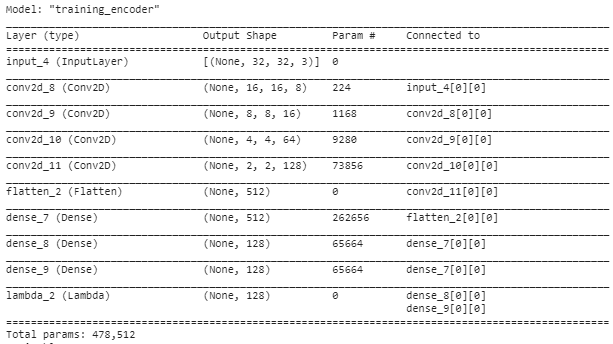
\includegraphics[width=\textwidth]{images/TrainingEncoder.PNG}
        \caption{Training encoder structure.}
    \end{subfigure}
    \begin{subfigure}[b]{0.49\textwidth}
        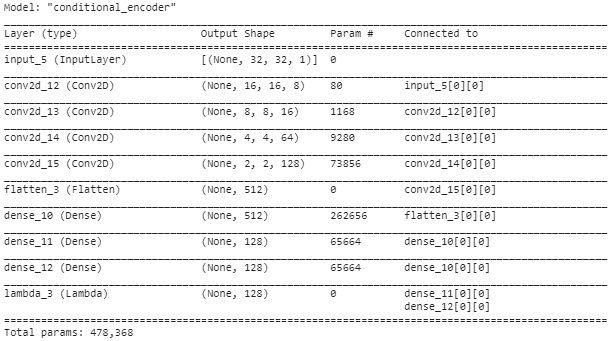
\includegraphics[width=\textwidth]{images/ConditionalEncoder.PNG}
        \caption{Conditional encoder structure.}
    \end{subfigure} 
    \begin{subfigure}[b]{0.49\textwidth}
        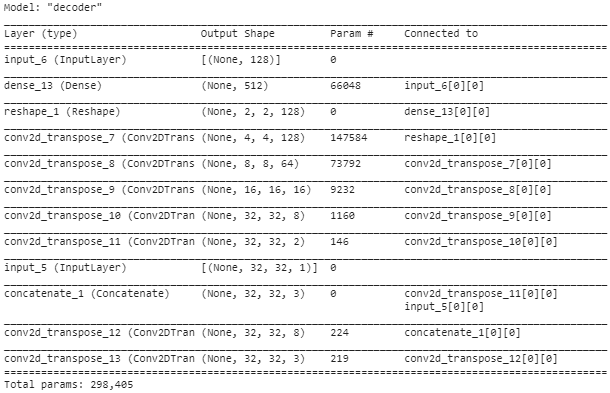
\includegraphics[width=\textwidth]{images/Decoder.PNG}
        \caption{Decoder structure.}
    \end{subfigure} 
    \caption{}
    \label{fig:cvae_model}
\end{figure}

\subsection{Hyper-Parameter Tuning}
Due to the lesser amount of time required to train the CVAE compared to the CGAN, its parameters could be feasibly tuned through repeated testing. 

The first parameter to be tested was the batch size, which for the CVAE is also dependent on Colab's available RAM, training time, and the value of the final training loss.
\begin{table}[H]
    \centering
    \caption{}
    \label{tab:operators}
    \begin{tabular}{llll}
        \textbf{Batch Size} &   \textbf{Loss after 100 Epochs}       &   \textbf{Training Time} \\   
        \texttt{1024}           &   \texttt{15.66}                   &   \texttt{55 sec}        \\
        \texttt{512}            &   \texttt{5.78}                    &   \texttt{1 min 6 sec}   \\
        \texttt{128}            &   \texttt{0.62}                   &   \texttt{1 min 22 sec}   \\
        \texttt{32}             &   \texttt{0.21}                   &   \texttt{3 min 8 sec}    \\
        \texttt{16}             &   \texttt{0.04}                   &   \texttt{5 min 42 sec}   \\
    \end{tabular}
\end{table}

As was the case for the CNN, lower batch sizes lead to a better final loss value but result in diminishing loss improvements at the cost of longer training times. The final batch size was 32, which seemed to offer a good balance between training time and performance.

The next parameter to be inspected was the latent dimension, which determines the size of the mean and standard deviation vectors of the latent feature space. VAEs with larger latent spaces are capable of storing more features. However having too large a latent dimension can cause overfitting as the optimiser model will be given too much space to store features in, leading to it memorising specific details of the training set. A latent dimension that is too small on the other hand will lead to the model underfitting because it lacks the storage necessary to memorise important general features. A variety of latent dimensions were tested  and compared in order to find an optimal size (see figure \ref{fig:vae_latent_dim}).

\begin{figure}[H]
    \centering
    \begin{subfigure}[t]{0.48\textwidth}
        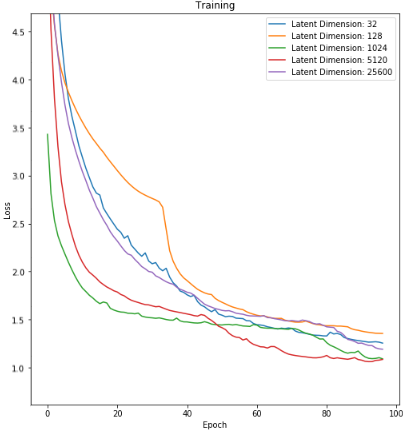
\includegraphics[width=\textwidth]{images/VAELatentDimensions.png}
        \caption{Effect of different latent dimensions on training the CVAE. A latent dimension in the range of 1024 to 5120 achieved optimal performance.}
        \label{fig:vae_latent_dim}
    \end{subfigure}
    \quad
    \begin{subfigure}[t]{0.48\textwidth}
        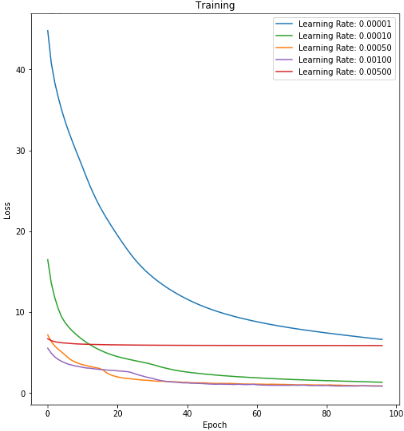
\includegraphics[width=\textwidth]{images/VAELearningRates.png}
        \caption{Effect of different learning rates on training the CVAE. A learning rate of 0.001 appears to be optimal, as larger values after that (0.005) seem to decrease performance.}
        \label{fig:vae_learning_rates}
    \end{subfigure} 
    \caption{}
    \label{fig:vae_hyperparameters}
\end{figure}

The tests showed that a latent dimension in the range of 1024 to 5120 achieved optimal performance, so 1024 was chosen as the final latent dimension as it was the smallest of the two and was more likely to only encode more important general features than a larger dimension would.

Adam was chosen as the optimiser, as it was clear at this point that it was the best choice for image colourisation models, considering how well it had worked for both the CNN and CGAN. A range of learning rates were tested on the CVAE (see figure \ref{fig:vae_learning_rates}) and it was found that a rate of 0.001 achieved the best continuous descent for both the training and validation losses and was thus used to train the final model.

%==================================================================================================================================
\chapter{Evaluation} 
In this chapter we will show colourisation results for each model and give an analyse the performance of each.

\section{Computation Time}
\label{computationtime}
To gain a better idea of how computationally expensive each model was, we evaluated the time it took for each one to train on a subset of Cifar10 to the point where they could produce sufficient results (see table \ref{tab:times}).

\begin{table}[H]
    \centering
    \begin{tabular}{ll}
        \textbf{Model} & \textbf{Training Time} \\   
        \texttt{CNN} & \texttt{9 min 41 sec} \\
        \texttt{CGAN} & \texttt{29 min 54 sec} \\
        \texttt{CVAE} & \texttt{2 min 45 sec} \\
    \end{tabular}
    \caption{Time required for each model to train on the Horse class of Cifar10.}
    \label{tab:times}
\end{table}

The CVAE proved to be the fastest model to train, followed by the CNN, both of which finished training in under ten minutes. The CGAN however, took considerably longer than both at almost half an hour. This is primarily due to the unique way which it needs to be trained compared to the other two models.

Training for the DCNN and the CVAE was always performed up to the point where the model began to overfit. This point was evident when the training and testing loss of each model began to diverge (see figure \ref{fig:dcnntime} and \ref{fig:cvaetime}). 

The CGAN however didn't have the same clear indicator for when training should end. Typically, the generator and discriminator's loss would continue to fluctuate around each other as long as training continued. At some point, either the generator or discriminator would begin to outperform the other, and their respective losses would start to consistently diverge (see figure \ref{fig:cgantime}). The CGAN was trained until this divergence became clear, which due to the inherent instability of the two loss functions, often required a large number of epochs to ensure the divergence was consistent and not the product of a momentary spike.

\begin{figure}[H]
    \centering
    \begin{subfigure}[b]{0.3\textwidth}
        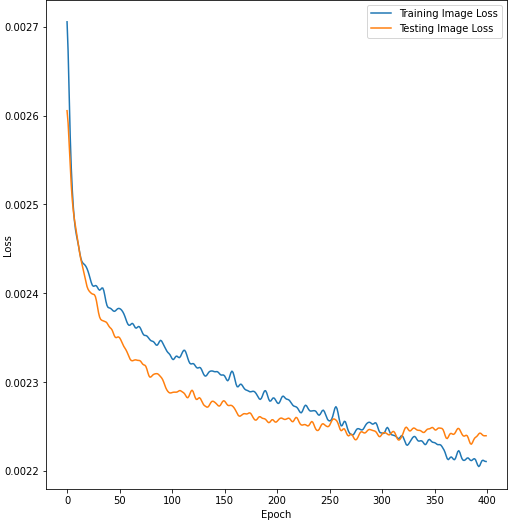
\includegraphics[width=\textwidth]{images/DCNNTime.png}
        \caption{DCNN learning curve. Training stops when the model begins to overfit.}
        \label{fig:dcnntime}
    \end{subfigure}
    \begin{subfigure}[b]{0.3\textwidth}
        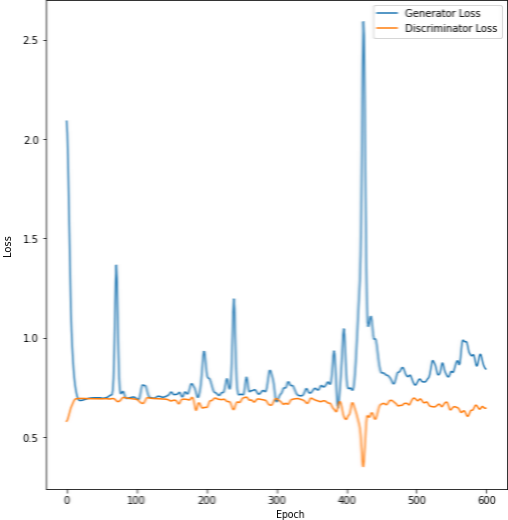
\includegraphics[width=\textwidth]{images/CGANTime.png}
        \caption{CGAN learning curve. Training stops when the loss of the generator begins to consistently diverge.}
        \label{fig:cgantime}
    \end{subfigure}
    \begin{subfigure}[b]{0.3\textwidth}
        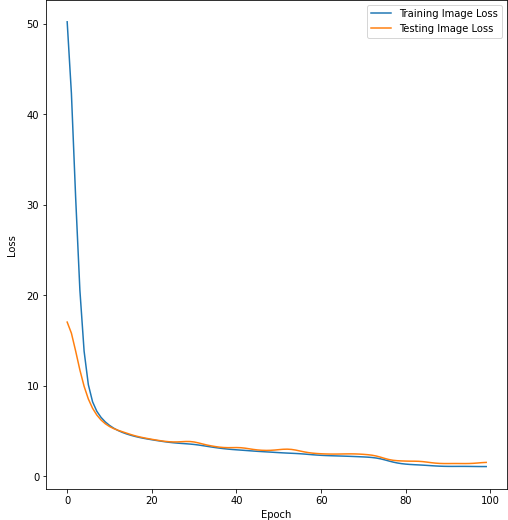
\includegraphics[width=\textwidth]{images/CVAETime.png}
        \caption{CVAE learning curve. Training stops when the model begins to overfit.}
        \label{fig:cvaetime}
    \end{subfigure}
    \label{fig:timeeval}
\end{figure}

\section{Feature-Based Colourisation}
\label{shapeseteval}

% NEEDS MORE EXPOSITION
To succinctly demonstrate the primary mechanism which Deep Learning models use to assign colours to areas of an image (explained in \ref{deeplearning}). The baseline CNN was trained on images from the custom Shape Set (see figure \ref{fig:shapeseteval}). 

\begin{figure}[h]
    \centering
    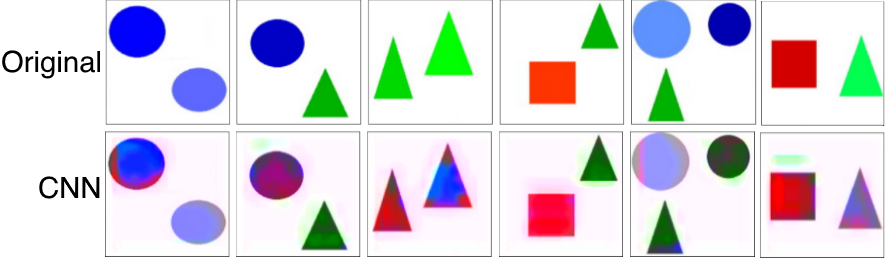
\includegraphics[width=1.0\linewidth]{images/ShapeSetEval.png}    
    \caption{Trained CNN results on unseen Shape Set images.}

    \label{fig:shapeseteval} 
\end{figure}

The CNN has learned that colours should only be present within the confines of shapes, and it has been able to identify particular shapes and how they correspond to specific colours. While it still has difficulty with some shapes, this is likely due to the variation in dimensions of the shapes themselves which leads to confusion, as well as the relatively small size of the dataset.

\section{Colourisation Results}

\begin{figure}[H]
    \centering
    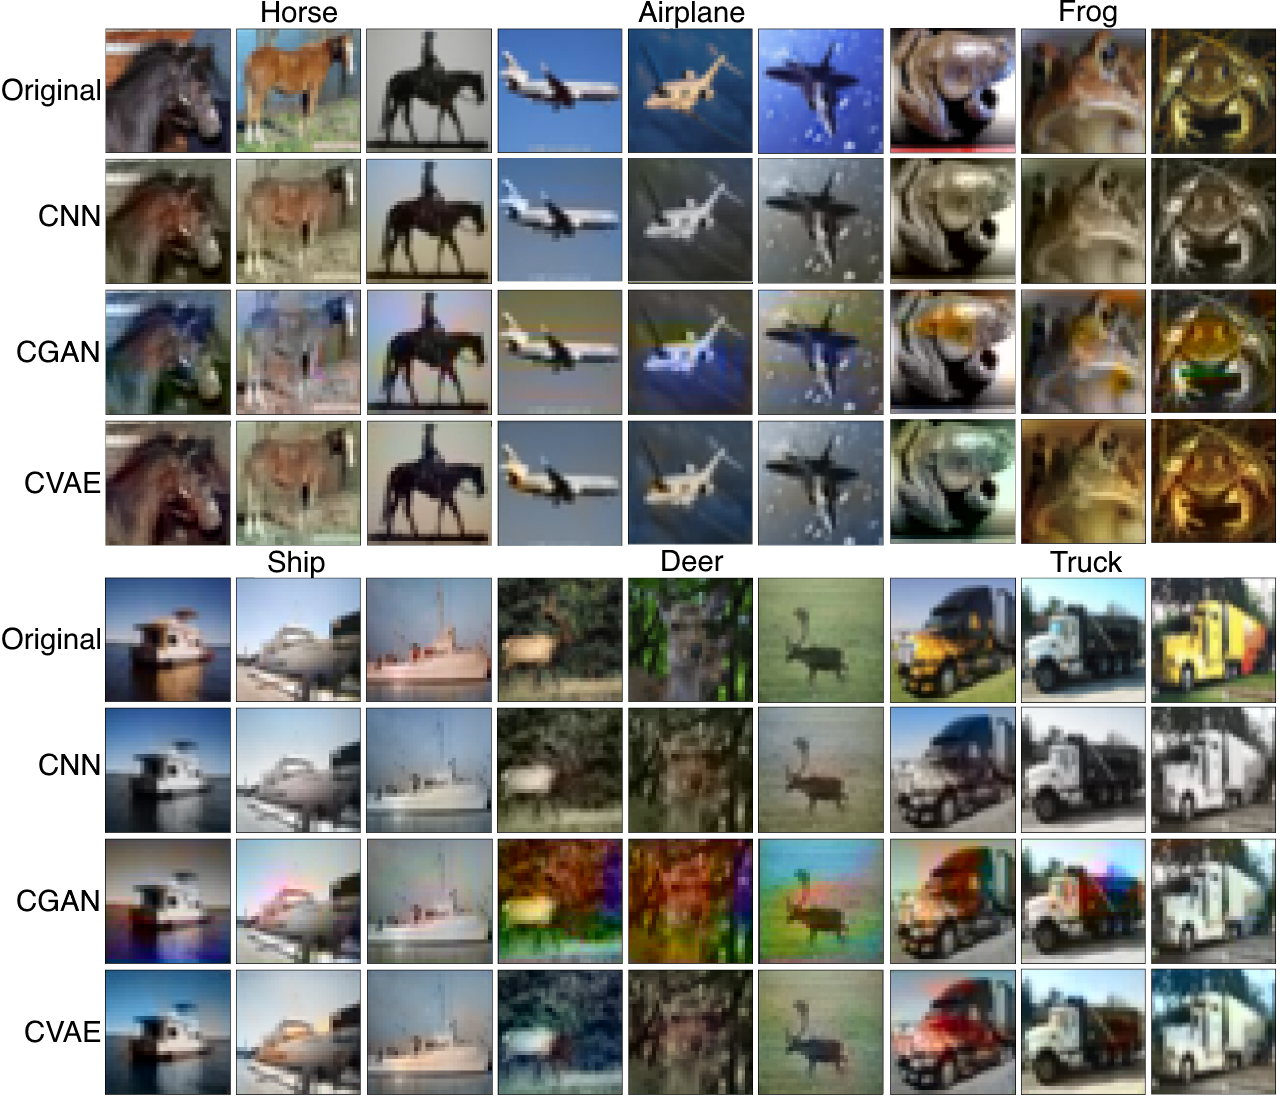
\includegraphics[width=1.0\linewidth]{images/Cifar10Eval.png}    
    \caption{Results on unseen Cifar-10 images from models trained for each specific class.}
    \label{fig:cifar10eval} 
\end{figure}

\begin{figure}[H]
    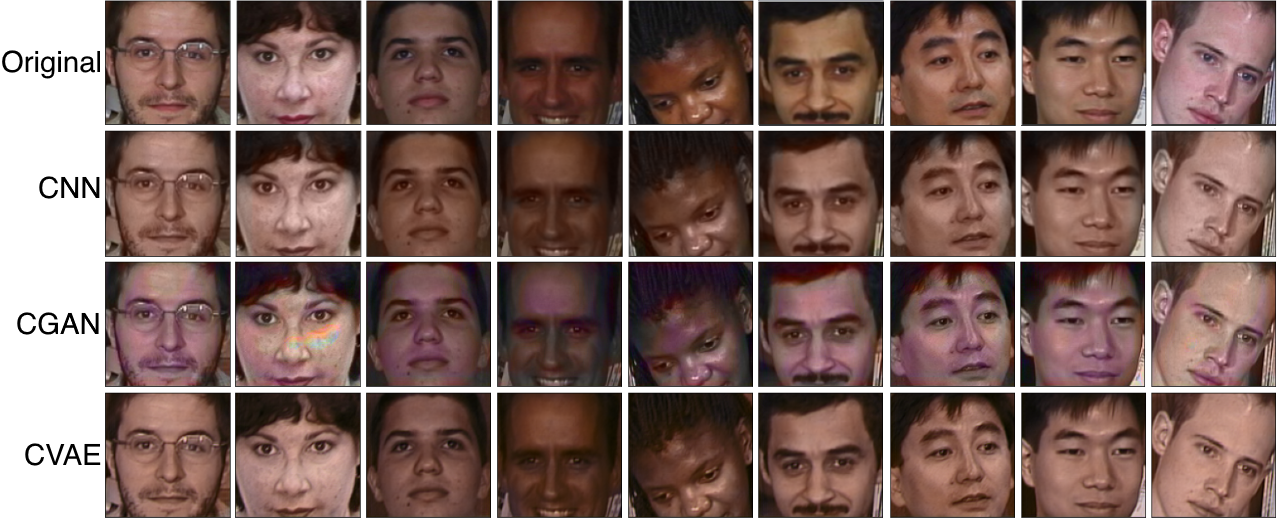
\includegraphics[width=1.0\linewidth]{images/FaceEval.png}   
    \caption{Trained model results on unseen Face images.}
    \label{fig:faceeval} 
\end{figure}

\begin{figure}[H]
    \centering
    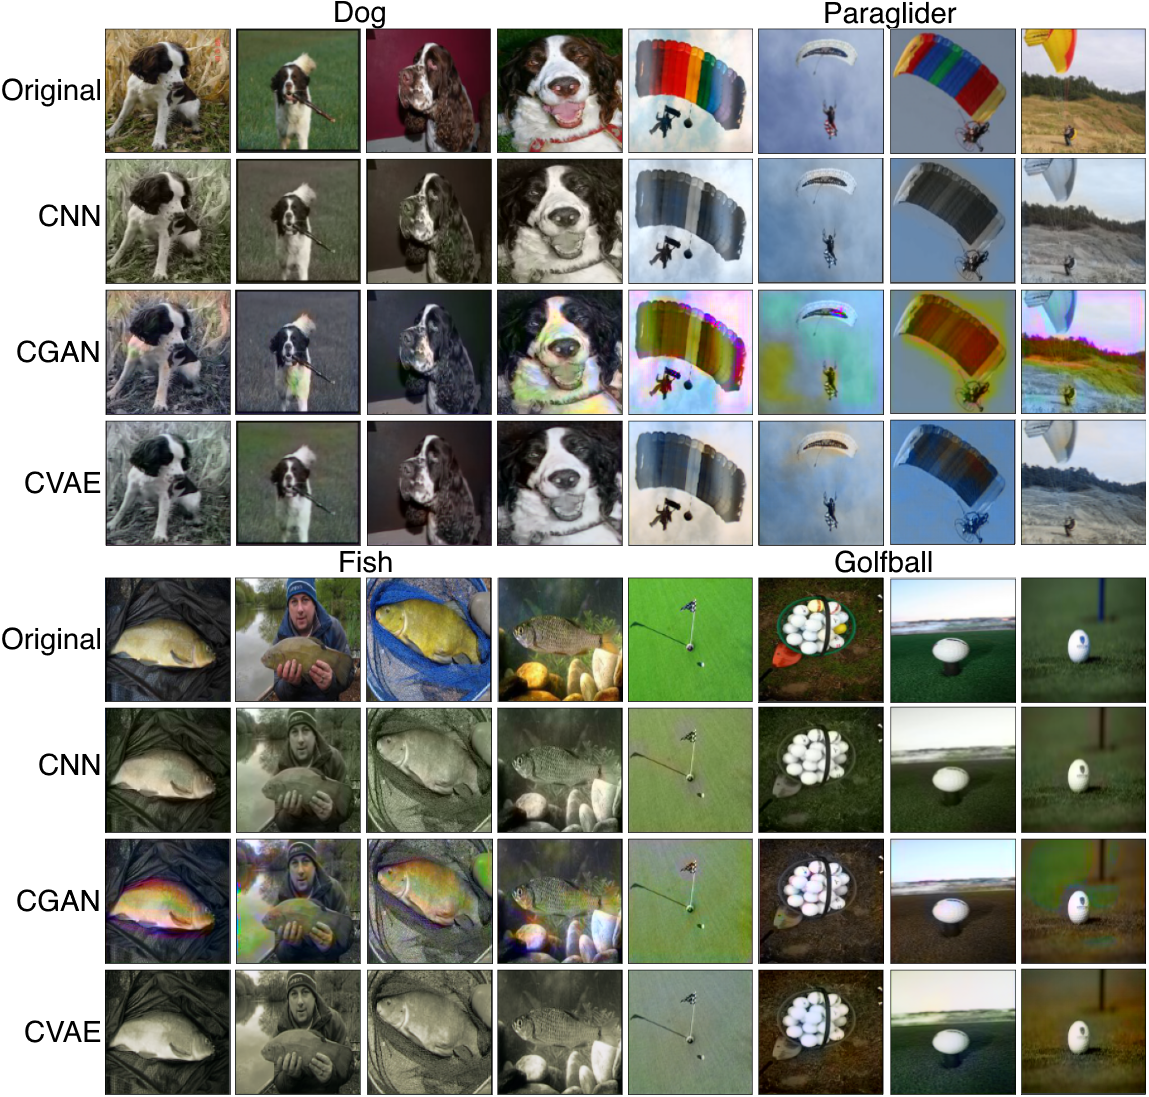
\includegraphics[width=1.0\linewidth]{images/ImagenetteEval.png}    
    \caption{Results on unseen Imagenette images from models trained for each specific class.}
    \label{fig:imagenetteeval}
\end{figure}

\textbf{N.B:} Every model was trained on each specific subclass of the Cifar10 and Imagenette datasets. This is because training on the entire dataset lead the models to produce results that are often too general, and made it difficult to determine the relative performance of each model. Training on the subclasses on the other hand, allowed the models to produce more useful detailed results that could help us identify in what particular areas the network may be failing. Certain classes also had interesting feature distributions that were worthy of closer analysis. For example Cifar10's Truck class was very varied and challenging, containing images with many different colours and characteristics. Compare this to the Deer class, which consistently contains images of deers in front of green vegetation, giving the network a chance to identify a very clear and prevalent feature.

\textbf{N.B:} The CVAE results are from a model with an unweighted reconstruction term. The CVAE results shown here are thus very similar to any other result it would have produced for a given image. This was done so as to not give the CVAE an unfair advantage compared to the other models by exploiting its ability to provide diverse colourisations, in order to achieve good outputs. 

\section{Discussion}

\subsection{CNN}

On Cifar-10, the CNN performed adequately on classes where clear and repetitive priors could be identified, for example always being able to colour the sky blue for the Ship class, or colour the background green for the Deer class. Where such clear priors weren't present however it tended to resort to using very muted colours, for example assigning neutral grey colours to the main components in the Frog and Truck classes. This shows how the CNN isn't very good at accounting for small details within images, and tends to colour features only after it has been provided with a large amount of clear priors encouraging it to do so. 

The CNN succeeded at producing plausible colourisations for the higher resolution Faces dataset, demonstrating that it is in fact capable of producing fairly detailed colourisation. Albeit, with the assistance of very constrained training data. 

For the more challenging Imagenette dataset, the CNN had some of the same issues it had with Cifar-10. It was again only capable of producing soft colour results, and could only apply colour to areas having clear repetitive priors, such as the sky for the Paraglider class or the grass for the Golfball class. 

The results demonstrate that the CNN is reliant on a great deal of clear prior information within its training data to allow it to provide strong colourisations to particular features, and that it tends to skip colouring details which it hasn't been provided enough training data relevant to. This makes it a very inconvenient solution to the problem, as to perform detailed colourisations it requires a large enough dataset tuned specifically to accomodate for the particular features it needs to recognise. One benefit however to the simplicity of the CNN's results is that it is more likely to not colourise a feature that it's unsure about, as opposed to colouring it incorrectly. Strong incorrect colourisations can result in very jarring and more obviously incorrect results, as was a major issue with the CGAN.

\subsection{CGAN}

For Cifar-10, the CGAN tended to use very saturated bright colours in its colourisations, which is contrary to the CNN's tendency to produce soft colours for difficult to determine features. Many of these colours are inappropriately placed however, which can be seen in its coloursations of the Plane and Deer class. This shows that the CGAN struggled a lot with edge detection compared to the CNN. 

On the Faces dataset it was able to better place colours on the image thanks to the more constrained nature of the dataset. However it had a similar issue with with its use of over saturated colours, assigning an unnatural purple tone to many of the faces.

For the Imagenette dataset however, the CGAN produced some surprisingly good results. In cases like the Fish and Paraglider classes, it still struggled with edge detection, however it was capable of producing the most detailed colourisations where the other two models were unable to assign almost any colours. 

The CGAN's issues with edge detection and colour intensity could be due to the fact that it is generalising too much and is accounting for many details which often aren't present. This is likely due to poor training and overfitting, considering how difficult it is to determine how long it needs to be trained for and what the optimal hyper-parameters are for it. The fact it was somewhat successful on a dataset as large and diverse as Imagenette however, could mean that it is best used when applied to problems with much more diverse priors in the training data, as opposed to the CNN's reliance on a large amount of specific priors. In either case, further evaluation on other datasets is required to determine the true cause of these problems, and major improvements are still needed in order to make the CGAN a viable solution for colourisation.

\subsection{CVAE}
\label{cvaediscussion}

The CVAE appeared to perform the best of all three models when colouring Cifar-10. It struck a good balance between providing plausible colourisations, while still being fairly detailed. Certain classes of images like the Truck and Frog had results containing strong colours that were well placed within appropriate features, showing the CVAE had overcome the CGAN's issues with edge detection and the CNN's issues with inadequate colours. It also performed well on the Faces dataset, being able to produce slightly sharper results than the CNN did.

On the Imagenette dataset it performed poorly however, suffering from the same issue as the CNN in that it failed to recognise certain features and resorted to using muted colours. In some cases it even did worse than the CNN, as can be seen in the Golfball class. This indicates that the CVAE is only proficient at handling data of a complexity it is designed for, and scales poorly to more challenging datsets with larger resolutions and more diverse features.

The CVAE's failure to colourise Imagenette images however isn't surprising considering it was designed and tested specifically on Cifar-10 data as were the other models. Its relative success with Cifar-10 is much more significant as it shows that it is the most capable model. It is clearly able to recognise the most features that can help it provide good results, while not accounting for too many that could lead to anomalies and poor generalisation.

A unique aspect of the CVAE also worth discussing is its ability to provide a variety of different colour outputs for a particular input. The CVAE with a low weighted reconstruction term was trained on the Frog class of Cifar-10 in order to demonstrate this ability (see figure \ref{fig:diverseeval}). 

\begin{figure}[H]
    \centering
    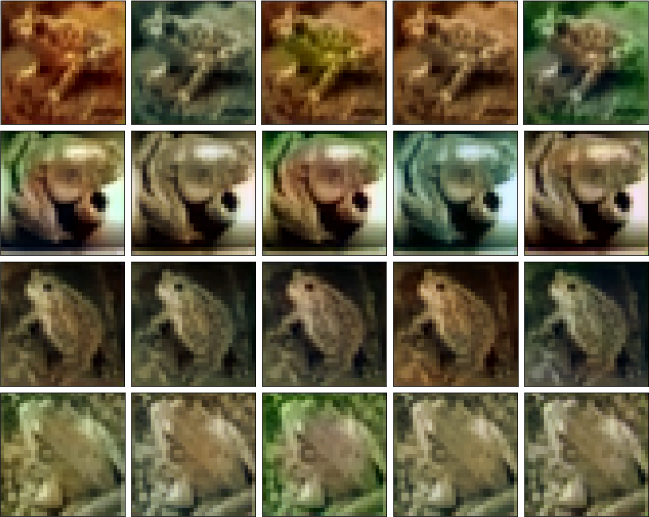
\includegraphics[width=0.7\linewidth]{images/DiverseEval.png}    
    \caption{Multiple outputs for Cifar-10 Frog images produced by a CVAE.}

    \label{fig:diverseeval} 
\end{figure}

%Maybe mention how this feature hasn't been fully developed
This feature alone may make the CVAE the most ideal tool for colourisation. A greyscale image may have a range of potential colourisations that could be considered acceptable, and the CVAE is capable of modelling this characteristic of the problem. Even if the CVAE can't model most of the colourisations that could be plausible, its ability to produce diverse outputs can still increase the likelihood of it providing good colourisation. The CNN and CGAN on the other hand are only capable of producing the same output for any given input after having been trained, meaning for some images they can fail completely, while the CVAE might still be able to produce a satisfactory result.

% \subsection{Sensitivity to Data}
% \label{sensitivitytodata}

% It's important to note that the characteristics of the training data had a much bigger impact on the quality of the results than the individual suitability of the model. This is always the case for ML projects however in the case of colourisation this issue is particularly impactful on the model's results due to the huge and unconstrained variety of potential priors. 

% The impact of this sensitivity can be seen in the colourisation results on the Faces dataset. This dataset is very well constrained and contains consistently present facial feature priors in each image, all presented very similarly as most faces are facing the direction of the viewer. As a result, even the CGAN which struggled the most with edge detection and feature recognition seemed to do well, showing how even a poorly adapted model can do well if given a good dataset.

% Each model was only trained on subclasses of the Cifar-10 and Imagenette datasets partly due to the difficulties arising from this sensitivity. The models could have in theory been designed to train well on the whole datasets, but that makes tuning them to perform well much more difficult. The models would have required even more priors in order to produce good outputs for such a large and varied amount of data, because such a large variety of information is likely to not be fully accounted far regardless of how deep a network is. A few state of the art projects such as \cite{DeepColorization} solve this by using feature extraction networks to provide high level feature information.
% Double check this source

%==================================================================================================================================
\chapter{Conclusion}    
% Conclusion Summarise briefly and fairly. Indicate what future work could be done, but remember: you won't get credit for things you haven't done.

% Analysed problem
% Analysed DL
% Analysed YUV and training data
% Designed 3 models
% Optimised hyperparameters of 2
% Tested on 3 datasets
% Discovered training data issues
% Discovered benefits of CVAE
% Still a long way to go

Our project investigated the use of Deep Learning to solve the problem of automatic image colourisation. We gave an in depth analysis of the problem itself and why DL in particular was an attractive solution. We then looked at how best to present the training data to DL models in the form of a YUV encoding, and we chose a range of datasets that would best help us train and evaluate our models. We implemented a CNN, CGAN, and CVAE for colourisation, and evaluated each of them on our datasets in order to determine which one was the most viable solution. 

Our CNN was designed from scratch and its architecture and hyper-parameters were optimised through repeated testing. We managed to produce a functioning colourisation model, however its results were often unimpressive. It relied on a large amount of clear priors for specific features within its training data in order to get it to recognise and colour them. When it failed to recognise features, it resorted to using muted colours which often resulted in grey and weakly coloured outputs. It is a potential solution, however in practice it isn't feasible that a user would need to produce a large and specific enough dataset to train it on, in order to get it to produce a good enough colourisation for a particular image.

The CGAN was implemented based mainly on suggestions from tutorials, as well as design decisions made on other colourisation CGAN models. This was due to the extensive amounts of time needed to train the CGAN relative to other models, which was a problem considering the project's time constraints, as well as the limited resources Colab provides. While the CGAN is used in a number of other projects for colourisation, and might well be a very viable solution, the colourisations from our model unfortunately weren't very good. It had major issues with edge detection, feature recognition, and colour choice, and requires further development in order to be a viable solution.

Our final model was the CVAE, which we were able to implement and tune through repeated testing better than the CGAN thanks to its ability to train very quickly. It produced very relatively detailed colourisations on our two simpler datasets, however began to perform poorly when applied to our more challenging data, even more so than the CNN. Its scalability issues aren't particularly bad howevever, as its difficulties with the challenging dataset can probably be overcome by increasing its capacity, considering it was designed primarily to colourise images from the simpler datasets which it did so well on. It also possessed the very useful ability of being able to produce a diverse range of potential colourisations for a given input. This makes it a very good solution considering how most greyscale images can have more than one plausible colourisation which the CVAE is more likely to account for. Its efficient training, ability to produce the most detailed results, and capacity for diverse colourisations, undoubtedly make it the most promising model of the three, and if time had permitted it would undoubtedly have been developed further.

\section{Future Developments}
\subsection{Better Training Environment}

Google Colab was a very limiting work environment for this project, and was one of the project's main constraints. Its requirement that a browser session remained open throughout training made training models over a certain capacity, and using large datasets almost impossible. An environment that provided the use of GPUs without these limitations, would allow us to do further work on resource and time intensive models like the CGAN, as well as allowing us to implement even higher capacity models that are trained on bigger datasets.

\subsection{Feature Extraction NNs}

As has already been demonstrated (see \ref{shapeseteval}), the primary mechanism which CNNs use to perform colourisation relies on feature extraction. To better guide this mechanism however, some state of the art projects like \cite{DeepColorization} also implemented dedicated feature extraction networks that fed feature data to the colourisation network, and this lead to better results. Our own CNN could probably have performed much better if more of the feature extraction work it struggled with was left to dedicated networks. It would have also been interesting to see what different impacts low, mid, and high level feature extraction networks would have had on performance, as well as how they could be combined.

\subsection{Disentangled CVAE}

Disentangled VAEs ($\beta$-VAEs) implement a hyper-parameter $\beta$ inside their loss functions which weighs how much the KL divergence is present in the loss. This weighting discourages correlation between neurons in the latent space, pushing each one to learn something unique about the input data\cite{BetaVAE}. It would have been interesting to see whether this had an improvement on the performance of the CVAE, as in theory it could have helped the model to more efficiently compress the most important features of the input data.

\subsection{Improving Diverse CVAE Colourisation}

The state of the art colourisation VAE \cite{DiverseColorization} further capitalised on the VAE's ability for diverse colourisation, by implementing the conditional encoder as a Mixture Density Network (MDN) that learns to map greyscale image data to multiple latent space embeddings. The MDN can take into account the one to many mapping between greyscale input and colour output, and allows the output latent representation to take multiple values conditioned on the same input. This provides a better selection of different latent embeddings to pass to the decoder. Their decoder's loss terms were also constructed in order to avoid blurry outputs and to take into account the uneven distribution of colours. These improvements would be worth trying on our own CVAE in order to improve its performance and its capacity for diverse outputs.

%==================================================================================================================================
%
% 
%==================================================================================================================================
%  APPENDICES  

\begin{appendices}

\chapter{Appendices}

\begin{figure}[h]
    \centering
    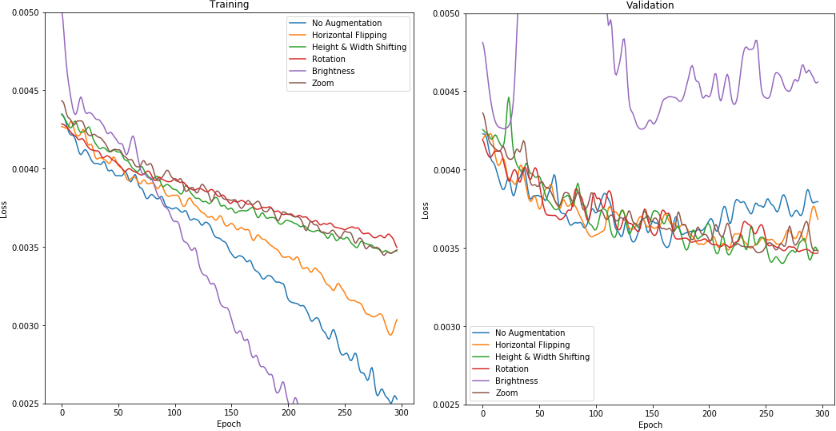
\includegraphics[width=0.9\linewidth]{images/AugmentationTesting.PNG}    

    \caption{Impact of different forms of data augmentation on network Training and Validation loss. Horizontal Flipping, Shifting, Rotation, and Zoom all had positive impacts on helping the model to generalise. Zoom was the only form of augmentation that worsened training.}

    \label{fig:augmentation_testing} 
\end{figure}

\begin{figure}[h]
    \centering
    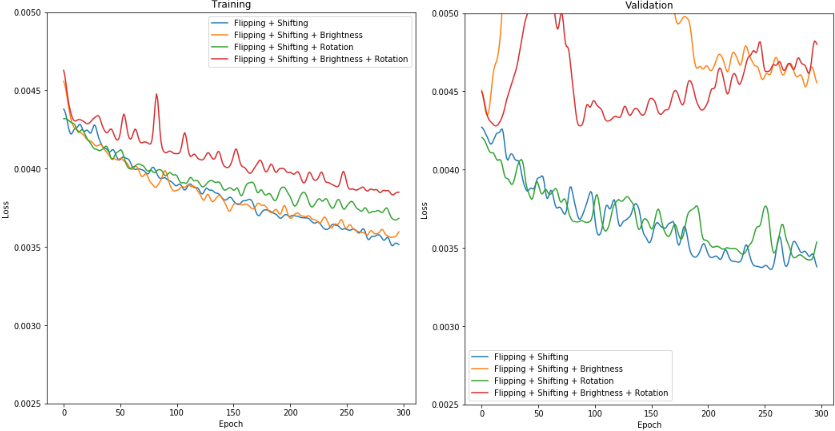
\includegraphics[width=0.9\linewidth]{images/AugmentationFurtherTesting.PNG}    

    \caption{Impact of combinations of data augmentation methods on network Training and Validation loss. Flipping + Shifting + Rotation allowed the training and validation loss to match each other most closely and thus was chosen as the final set of augmentation techniques.}

    \label{fig:augmentation_futher_testing} 
\end{figure}

\begin{figure}[h]
    \centering
    \begin{subfigure}[b]{0.5\textwidth}
        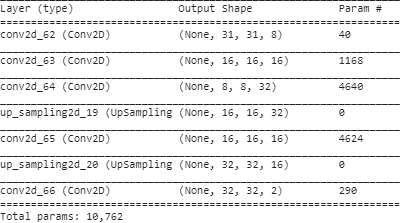
\includegraphics[width=\textwidth]{images/ShallowModel.PNG}
        \caption{}
    \end{subfigure}
    \quad
    \begin{subfigure}[b]{0.41\textwidth}
        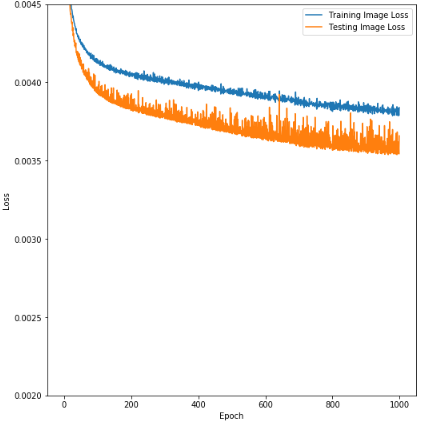
\includegraphics[width=\textwidth]{images/LowCapacityLoss.PNG}
        \caption{}
    \end{subfigure} 
    \caption{Low capacity shallow model designed for a 32x32 Cifar-10 input set with accompanying loss. The network is far too simple to be a feasible colourisation model however it does serve as a good start to analyse how poorly it performs in order to see how far the structure is from being a viable model. The model is incapable of storing enough information past a certain epoch and thus the loss for both training and validation data plateaus meaning a higher capacity model is needed.}
    \label{fig:shallow_model}
    \vspace{10mm}
    \begin{subfigure}[b]{0.5\textwidth}
        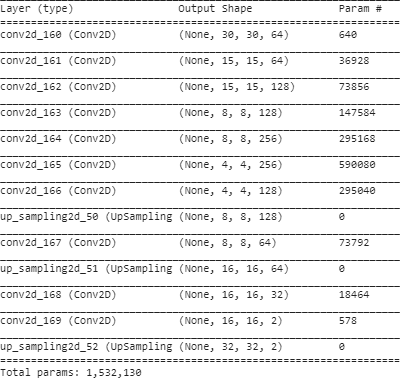
\includegraphics[width=\textwidth]{images/DeepModel.PNG}
        \caption{}
    \end{subfigure}
    \quad
    \begin{subfigure}[b]{0.41\textwidth}
        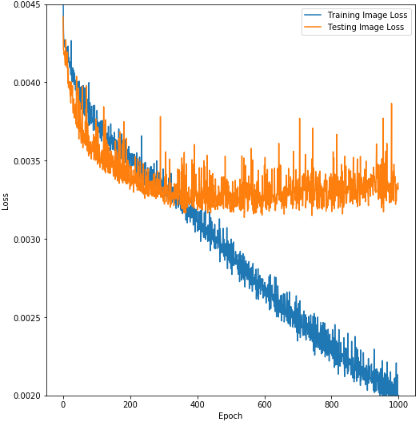
\includegraphics[width=\textwidth]{images/HighCapacityLoss.PNG}
        \caption{}
    \end{subfigure} 
    \caption{The contrasting deep model also designed for Cifar-10's 32x32 set with accompanying loss. The network is much deeper and downsamples the image to an even lower 4x4 resolution over more convolutional layers. The number of parameters here is excessive relative to the detail of the set and, while it will produce a detailed output for the training set, will inevitably overfit and be unable to generalise to unseen images. The loss for the training data continues to decrease however the loss for the validation data plateaus and gradually starts to go up again, meaning the model is overfitting and is memorising information from the traning data.}
    \label{fig:deep_model}
\end{figure}

\end{appendices}

%==================================================================================================================================
%   BIBLIOGRAPHY   

% The bibliography style is abbrvnat
% The bibliography always appears last, after the appendices.

\bibliographystyle{abbrvnat}

\bibliography{l4proj}

\end{document}
